% !TEX root = ../main.tex
%
\chapter{Analysis}
\label{sec:4}

\cleanchapterquote{To see a World in a Grain of Sand \\
                   And a Heaven in a Wild Flower \\ 
                   Hold Infinity in the palm of your hand \\
                   And Eternity in an hour}{William Blake}{(Auguries of Innocence)}

In this chapter the details on data sample and the analysis technique used for the search of the \dst
dibaryon and the related antiparticle, will be presented. 
The \dst has been searched in the \dstdecay decay channel, since this is expected to be the
most relevant channel \ -- the expected branching ratio is around 23\% -- \ detectable by the
ALICE apparatus.

From now on, the \dst dibaryon will be identified as \ds as well as \dst, while the deuteron
will be also called $d$.

%
%
\section{Analysis strategy} \label{sec:4.1}

In this section more details are given on the strategy that was decided to use to search the
\dst dibaryon. 
The strategy is to perform a \textbf{blind analysis} for the invariant mass distribution
(\minv) of the \dst \textit{candidates}. A \ds \textit{candidate} is a triplet composed 
by the \ds decay products, or the related antiparticles, in the considered decay channel.
A region of interest, where the \ds signal is expected to be, has been defined:
\begin{center}
\textbf{Region of Interest (RoI)}\  $\rightarrow$ \  $(2.280  < $\ \minv$  < 2.480)\ $ \gevcs.
\end{center}
The RoI, will not be considered while studying the selections.
When the selections are satisfactorily optimized the RoI will be \textit{unblinded} and a
background subtraction will be performed to look for the signal.

The idea behind the blind analysis is to optimize the selections and to develop a model
able to describe the background of the measurement without introducing any bias. 

The predicted physics properties of the \dst are summarized in the table \ref{tab:dst_prop}. 
Considering these values, the chosen RoI ensures that the signal \ -- if it exists and it is visible
-- \ is basically in that mass interval.
\begingroup
\renewcommand{\arraystretch}{1.5} % Default value: 1
\begin{table}
\centering
\captionsetup{justification=centering}
\begin{tabular}{lr}
\multicolumn{2}{c}{\textbf{Predicted properties}}      \\
\toprule
Mass				             & 2.380 \ \gevcs 	    \\
$\Gamma$			        	 & 0.070 \ \gevcs 	   	\\
$d\; \pi^{+} \pi^{-}\ $ B.R.	 & 23(2)\ \%		    \\
\midrule
\end{tabular}
\caption{\dst predicted properties.}
\label{tab:dst_prop}
\end{table}
\endgroup

%
%
\section{Data and Monte Carlo sample} \label{sec:4.2}

The analysis presented in this thesis is based on the \pPb collisions at \sctev 
collected in 2016. 

The sample of collected data consists of nearly $5.5\times10^{8}$ minimum bias events.
In order to increase the number of collected events during this data taking period, two
different minimum bias trigger has been adopted.
The first trigger, called \code{CENT}, basically is a minimum bias trigger for the central barrel
detectors. The SDD detector has a greater busy time than other detectors \ -- around three times
than SSD -- \ which limits the rate of collected events. 
In order to increase the rate of collected events, the second trigger, called \code{FAST}, allows
to detect events coming in the SDD busy time by excluding the SDD by the acquisition.
The data flow and triggers management is performed by the ALICE CTP (Section \ref{sec:data_flow}).

In the \textit{off-line} event reconstruction the whole data set analyzed in this work has been
reconstructed excluding the SDD information from the process, in order to made compatible
the data acquired with the two different triggers.

For this analysis two different Monte Carlo data sample has been used.
The first one is a sample of $\sim 5 \times 10^{5}$ \pPb events with injected exotic states
and has been used to study the \dst properties and the reconstruction efficiency of its decay.
The second one is a sample of $\sim 4.6 \times 10^{7}$ \pPb events and has been used to study 
the properties of the background sources of the measurement.

The Monte Carlo data are based the EPOS-LHC generator \cite{epos_lhc} which is an event 
generator for minimum bias hadronic interactions, used for both heavy ion interactions and cosmic 
ray air shower simulations.
Since the EPOS-LHC does not include any (anti-)dibaryon, an \textit{ad-hoc} generator was used to
inject \ds and \dsbar on top of each EPOS-LHC event in the first Monte Carlo sample.
In each generated event are injected ten \dst and ten $\ensuremath{\bar{{d}^{*}}(2380)}$, 
with a homogeneous distribution in transverse momentum \ -- in the $0 \leq \pt \leq 8\;\gevc$ interval
-- \ as well as in the azimuthal angle $\phi$ and in rapidity.
The injected \dst are made decay by the generator through the \dstdecay channel. 

The other possible decay of the \dst have not been considered since are not relevant or not
detectable \ -- because of the presence of neutral particle in the final state -- \ by ALICE.
Since the considered decay occurs through Strong interaction, the decay takes place basically in the 
interaction vertex. Therefore the decay products are generated starting from the interaction vertex
together with the others collision products.

The transport code used for the generation of the detector response \ -- as described
in section \ref{sec:} -- \ is GEANT? 
The data taking conditions are accounted in the MC by reproducing the configuration of the different 
detectors in the runs used for the analysis.

\subsection{Monte Carlo validation} \label{sec:4.2.1}

As mentioned above, the EPOS-LHC event generator does not include the \dst dibaryon, therefore it has
been injected on top of \pPb collision. 
The first thing done in this thesis is the validation of the injection process through
the analysis of the resulting events.
This validation ensure that the injected dibaryonic states have the correct physics properties
expected for the \dst.

This validation has been done checking the shape of the invariant mass distribution of \dst decay 
products, taking the generated tracks. Only tracks from a true \dst and belonging to the same 
mother has been considered, in order to avoid background. 

\begin{figure}
    \centering
    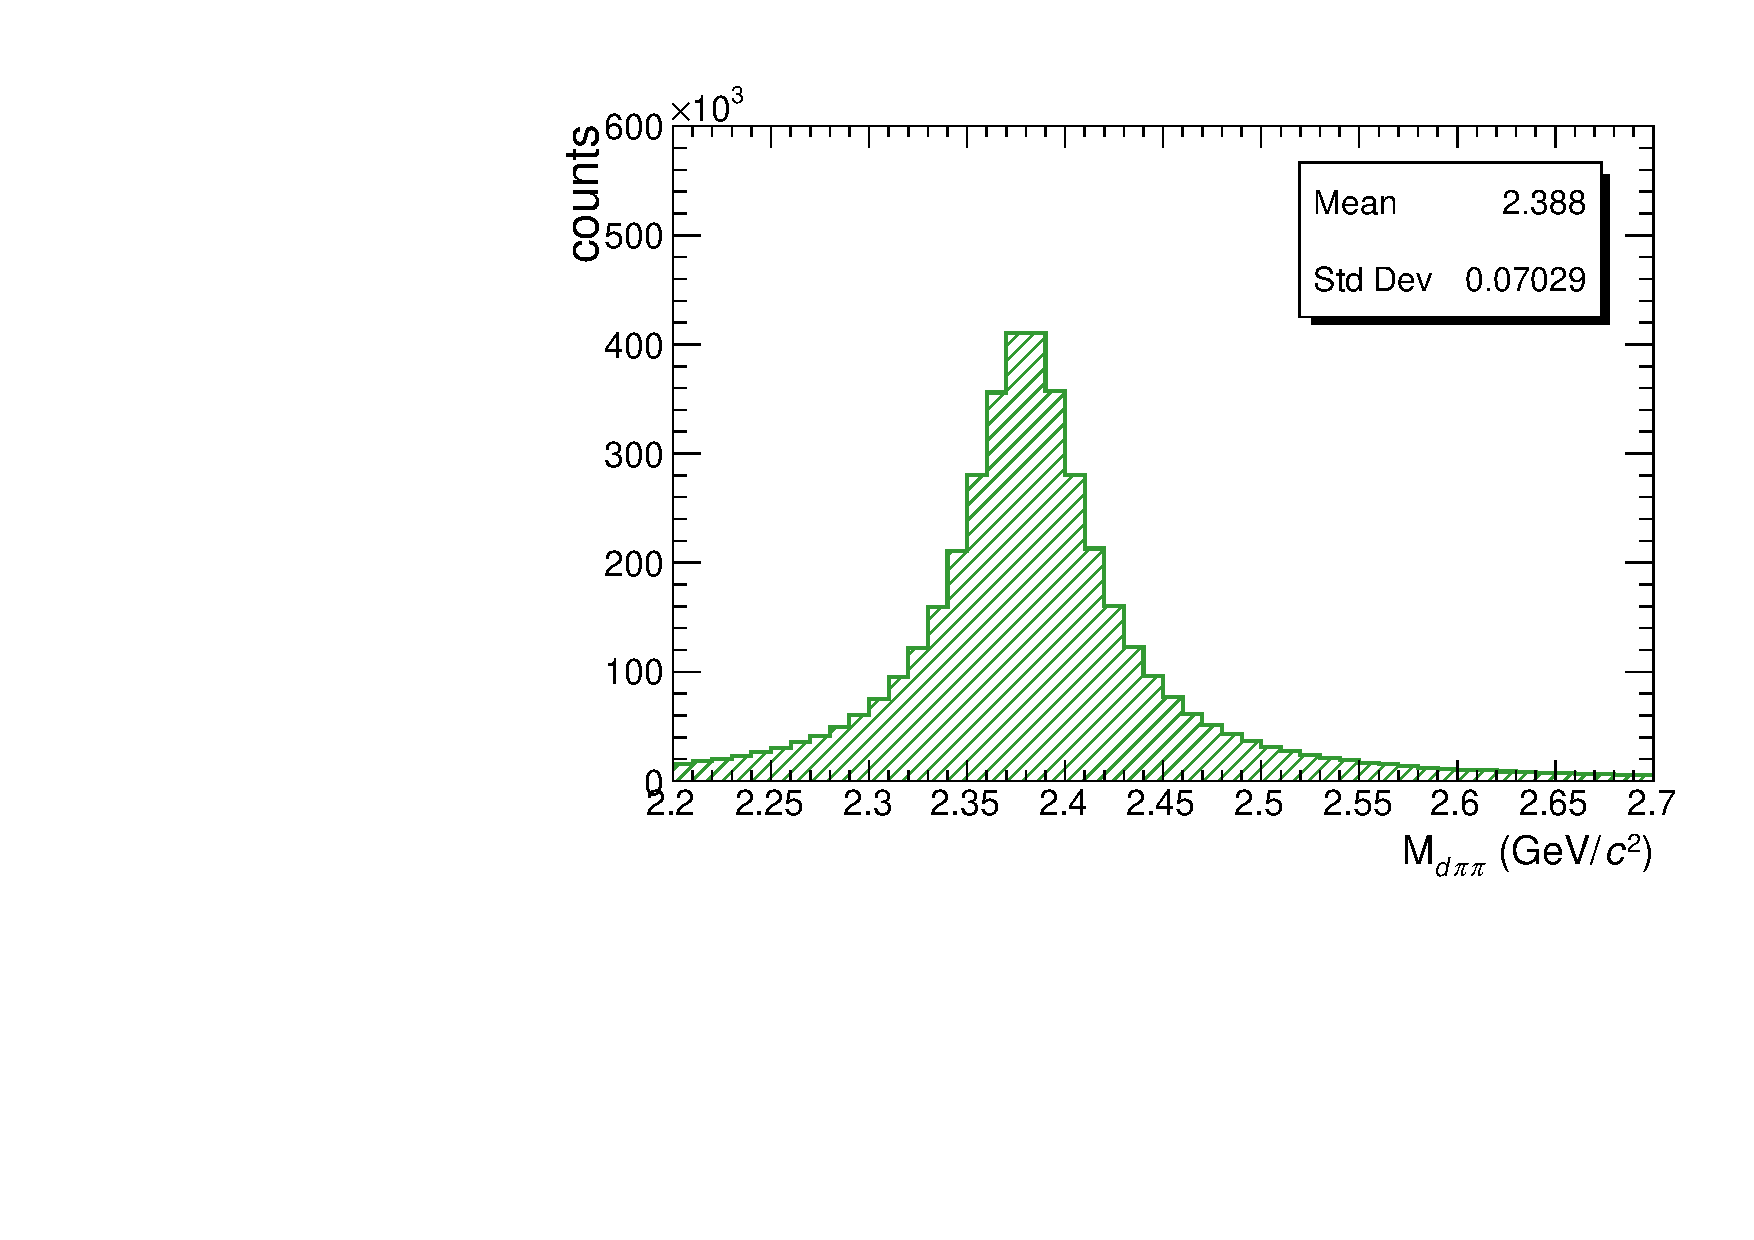
\includegraphics[width=0.6\textwidth]{gfx/valid}
	\caption{Invariant mass distribution of the \dst decay product, obtained using the generated tracks. The distribution shows the correct shape. The mean and the \textit{rms} of the distribution are compatible with the predicted properties of the \dst.}
	\label{fig:valid}
\end{figure}

The signal observed by the WASA-at-COSY collaboration, as discussed in section \ref{sec:wasa}, has
mass of 2380 \mevcs and a width of $\sim$ 70 \mevcs. Therefore, Figure \ref{fig:valid} shows that the
injected signal has the correct features of the \dst.

%
%
\section{Event and track selection} \label{sec:4.2}

In this analysis, the events are analyzed with the \code{CODEX} framework\footnote{The \code{CODEX} 
framework is part of the \code{AliPhysics} software (Section \ref{sec:anal_frame}) and it is 
specifically developed in order to provide analysis tools for the ALICE analysis related to nuclei
production.} that allows to select events with certain features and to store them in a compressed
format.
Such compressed data can be stored and analyzed on local machines, providing an easier and faster 
analysis chain.

Using the \code{CODEX} framework the event and track selection takes part in two different stages.
In the first stage the \code{CODEX} analyze the considered data sample on the WLCG (Section 
\ref{sec:offline}) filtering and storing interesting events in a compressed format. 
Basically, it works as an \textit{off-line} trigger.
In the second stage the filtered data are analyzed on local machines and further track
selections are applied.
In the following sections more details on the event and track selection are provided.

%
\subsection{Event selection: \code{CODEX} filtering}

In the \code{CODEX} filtering the event selection it is done in two steps.
In the first step events are selected using standard ALICE requirements for \pPb events: 
a pile-up rejection exclude events with more than one primary vertex and
a selection based on some features of the primary vertex guarantees the goodness of the
reconstructed vertex.
This last selection, basically reject events for which the vertex reconstructed with full tracks
differs to much from the vertex determined with the SPD only.
More details on the two vertexing processes are given in Section \ref{sec:vertexing}.
The selections applied to the primary vertex in this step are summarized in Table \ref{tab:cod_sel1}.

\begingroup
\renewcommand{\arraystretch}{1.5} % Default value: 1
\begin{table}[hb]
\centering
\begin{tabular}{lr}
\multicolumn{2}{c}{\textbf{Event selection in \code{CODEX}}}        \\
\toprule
$\mid \textit{z} \mid\ $ primary vertex            & $<$ 10 cm      \\
\textit{z}$_{SPD}$ vertex resolution               & $<$ 0.25 cm    \\
$\mid \textit{z}_{SPD} - \textit{z}_{Track} \mid$  & $<$ 0.5 cm	    \\
\midrule
\end{tabular}
\caption{This early selections made in the first step of the \code{CODEX} process ensure a good reconstruction of the primary vertex.}
\label{tab:cod_sel1}
\end{table}
\endgroup

In the second step a track and particle identification selection with loose cuts is performed.
The concept is to store locally only events with a \textit{(anti-)deuteron candidate}, since without
the (anti-)deuteron the \dst decay can't be reconstructed.
The rate of expected (anti-)deuterons in \pPb inelastic collisions is approximately $10^{-4}$,
therefore with this selection it is possible to reduce the number of stored events from at least four
order of magnitude, making the data sample manageable on local machines.

Following the $n\sigma\ $ technique described in \ref{sec:PID}, a track with 
$n\sigma_{TPC} < 5$ and $n\sigma_{TOF} < 10$ for tracks with $\pt > 1.5\; \gevc$,
respect to the deuteron mass hypothesis is considered a \textit{(anti-)deuteron candidate}.
Only events with at least one \textit{(anti-)deuteron candidate} are stored.

%
\subsection{Track selection} \label{sec:track_sel_crit}

In the second stage the filtered data are processed on local machines, in order to define
the best possible track selections.
Having locally the whole data set of interesting events allows to process the data very 
quickly and therefore to study and to test further track selections easily.
In the following the final selections, established after many attempts, will presented.

Since \dstdecay is a strong decay only tracks coming from the primary vertex are 
considered in this analysis. Therefore a selection on the DCA \ -- defined in Section
\ref{sec:vertexing} -- \ has been applied. 
The other selections are related to track parameter which describe, somehow, the goodness of the
reconstruction process of the track. 
In order to use only the geometrical region where the ALICE experiment is able to perform a full
tracking and to provide the best possible PID information, only tracks in the pseudorapidity 
region $|\eta| < 0.9 $ are selected. This requirement is mainly related to the TPC acceptance,
since it is the main used detector. 
Moreover, to guarantee a track momentum resolution better than 5\% and a TPC \dedx resolution of
6\%, the selected tracks are required to have at least 70 clusters in the TPC.
Then the selected tracks are required to overcome successfully the ITS and the TPC refit process
\ -- described in Section \ref{sec:tarcking}.
In addition, the $\chi^{2}$ per TPC clusters is computed in the track fitting procedure and is
required to be less than 4, while the \textit{Golden $\chi^{2}$} \ -- defined as blah blah blah -- 
\ is required to be less than 36.
Finally, further selection is applied on the \code{kKink} parameter in order to reject
particles coming from beam line interactions.

\begingroup
\renewcommand{\arraystretch}{1.5} % Default value: 1
\begin{table}
\centering
\begin{tabular}{cc}
\multicolumn{2}{c}{\textbf{Track selection criteria}} \\
\toprule
Variable                            &   Selection        \\
\midrule
$\mid \eta \mid$  				    &	$\leq$ 0.9	     \\
TPC clusters	                    &	$>$ 70		     \\
$\chi^{2}$ per TPC clusters		    &	$<$ 4		     \\
Golden $\chi^{2}$                   &   $<$ 36           \\
TPC refit					        &	\code{true}		 \\
ITS refit						    &	\code{true}		 \\
Kink daughters			       		& 	rejected		 \\
DCA$_{xy}$					        &	$<$ $(0.0105+0.0350) / \ensuremath{\pt}^{1.1}$  cm \\
DCA$_{z}$					        &	$<$ 2 cm    	 \\
\midrule
\end{tabular}
\caption{Summary of the track selections applied in the analyses of the 2016 data sample.}
\label{tab:tselection}
\end{table}
\endgroup

The aforementioned track selection criteria are applied to all the analyses presented in this
thesis and are summarized in Table \ref{tab:tselection}

%
% 
\section{Reconstruction of the \ds} \label{sec:ds_candidate}

After the event and track selection there is nothing left but to determine the (\dsbar)\ds candidates.
This is done by selecting the daughter tracks of the two charged pions decay:
\begin{equation}
    \dstdecay.
\end{equation}
Therefore a (\dsbar)\ds candidate is a triplet of tracks identified as (anti-)deuteron, \pip and
\pim.

The determination of the particle species of the track is performed with a track-by-track
selection on the $n\sigma$ variable as described in Section \ref{sec:PID}. One of the main
challenges in this analysis is to be able to have a good identification of the deuteron in the 
momentum range in which the \ds production is expected to be more abundant. % \ -- $m_{d} >> m_{\pi}\ $ implies that most of the \ds 
% momentum is taken by the deuteron, therefore the deuteron. 
But, at the same time,
it is essential to have a high purity of the pions and deuterons samples.
Therefore the choice of the detectors which are to be used for the PID is not trivial and should
be investigated.

\begin{figure}
    \centering
    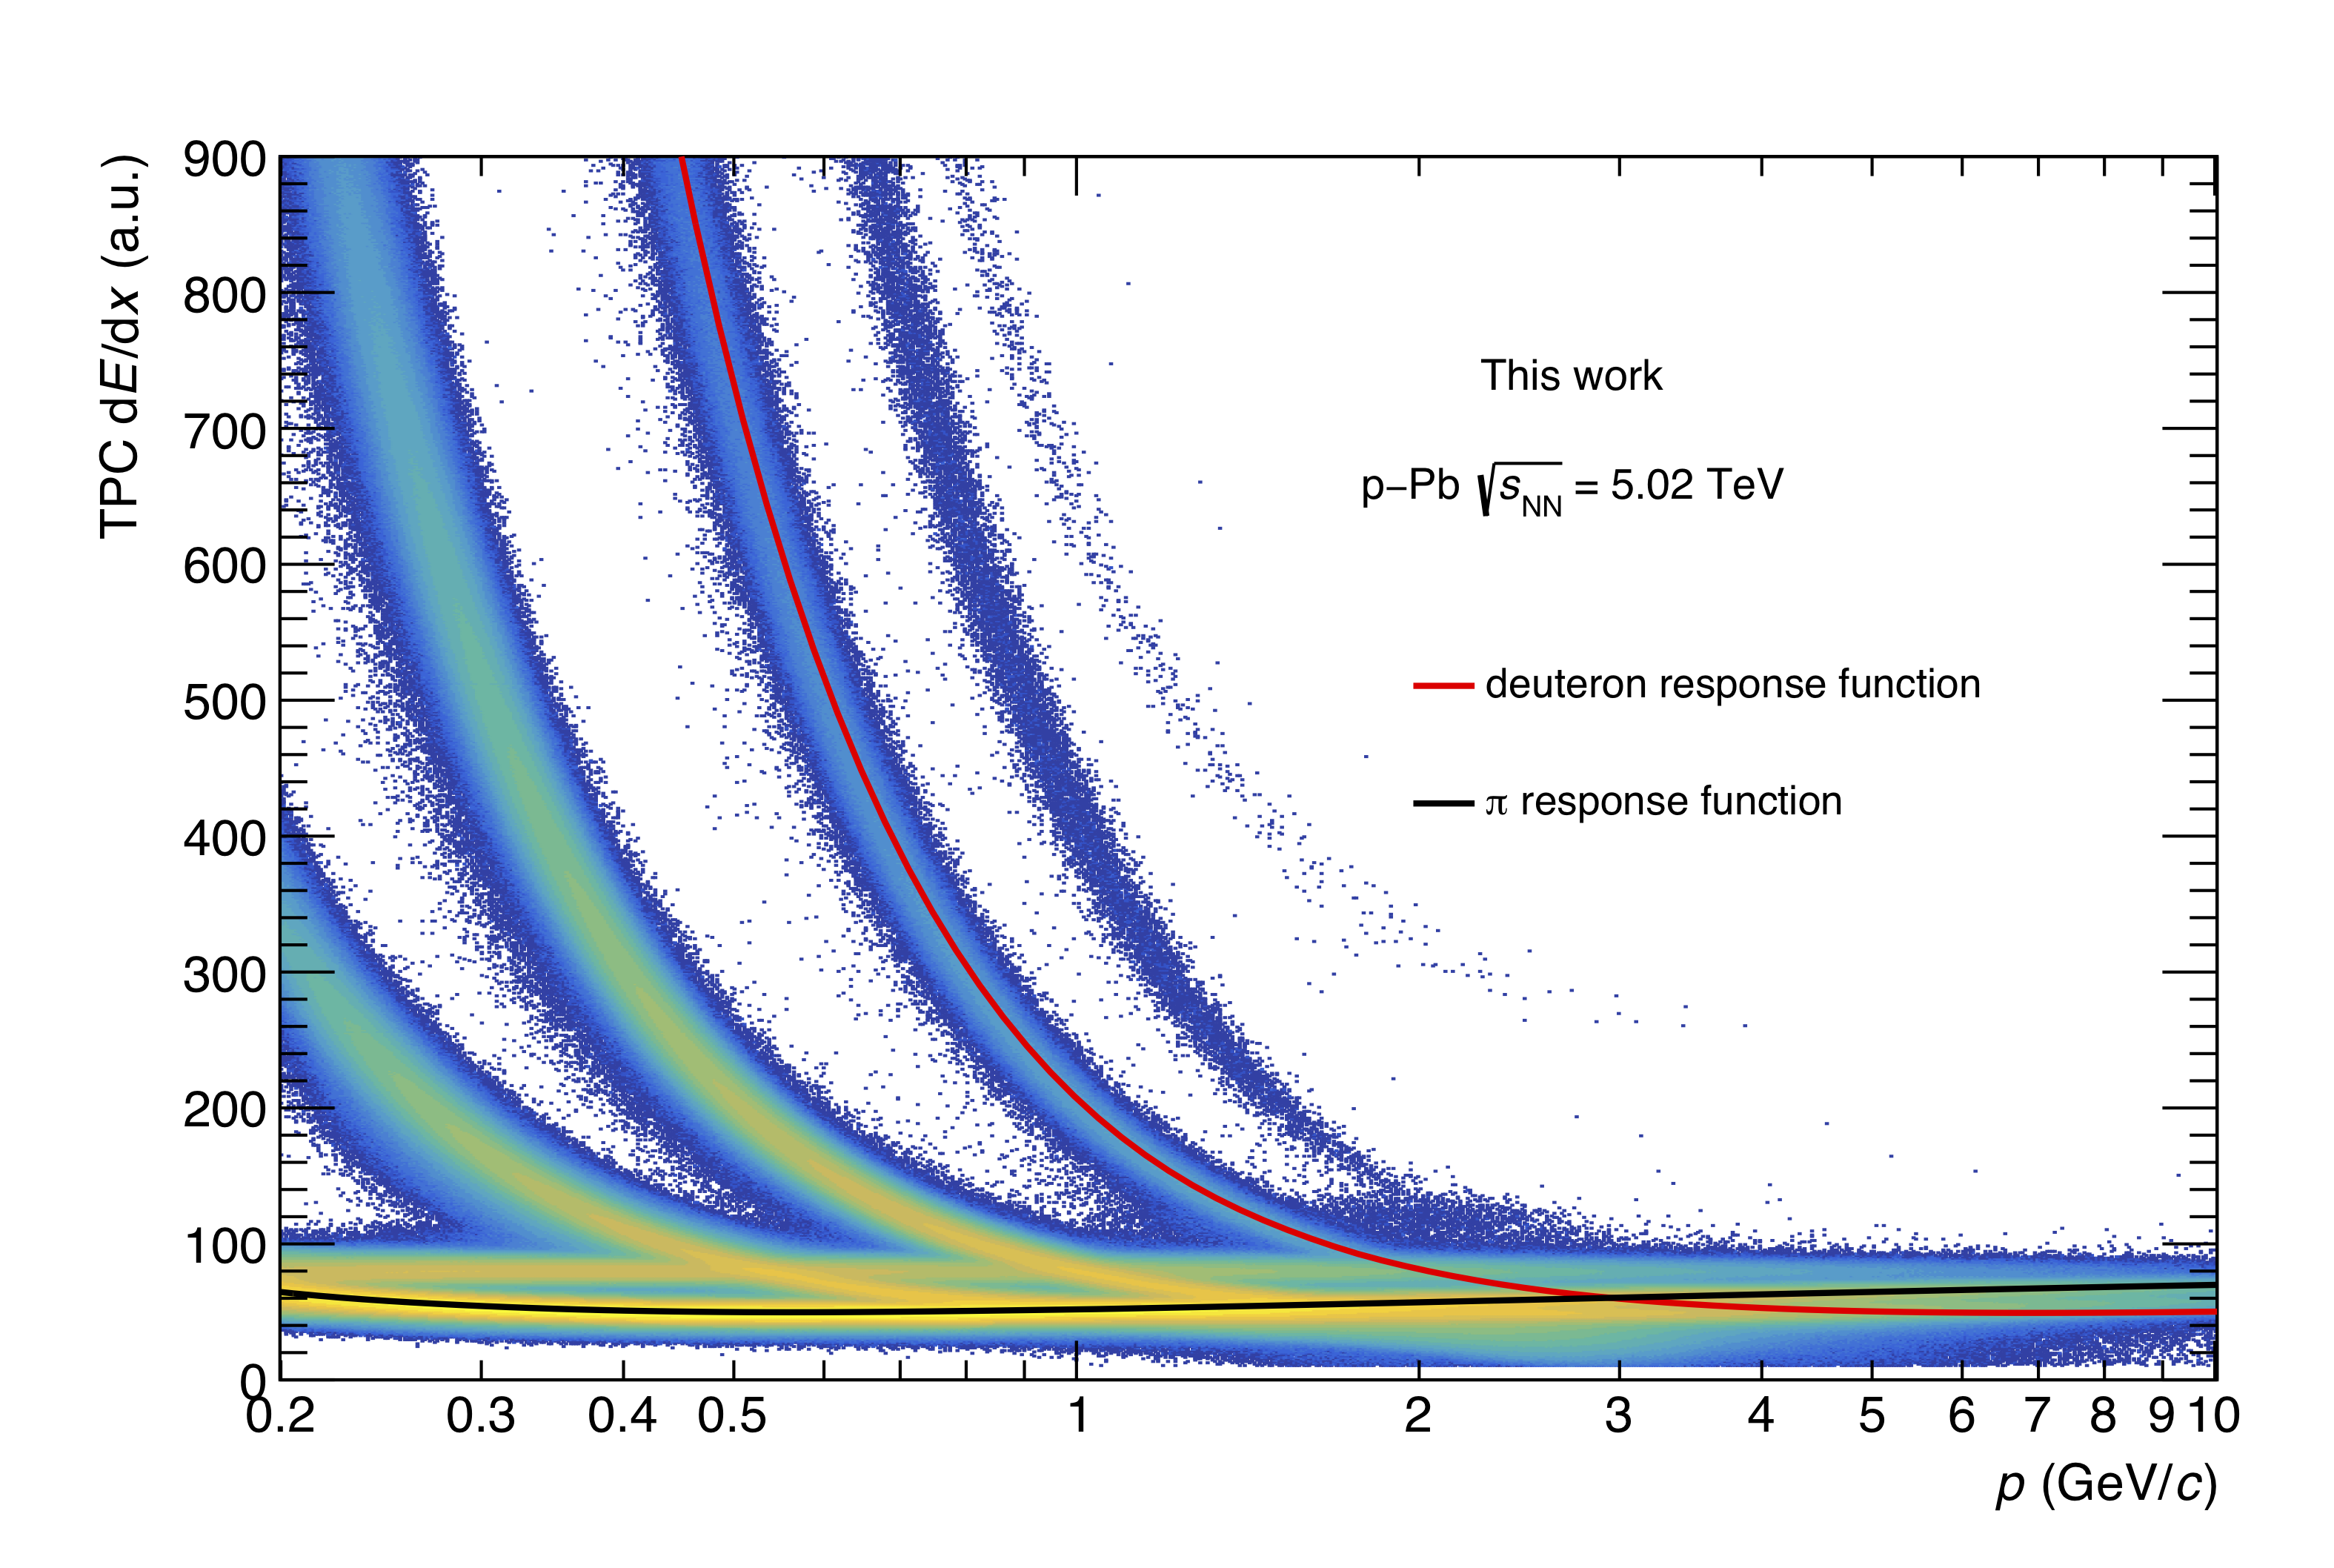
\includegraphics[width=0.8\textwidth]{gfx/pid_tpc}
	\caption{Specific energy loss in the TPC active volume as a function of the particle rigidity in \pPb collisions for the 2016 data sample. The solid lines represent the expected TPC response for pion (black) and deuteron (red).}
	\label{fig:tpc_pid_this}
\end{figure}

A clear identification of the (anti-)deuteron using the TPC information only, is possible for
tracks up to $p \sim 1.2\; \gevc$ due to the finite resolution on the specific energy loss measured by
the TPC and the contamination from electrons and positrons (Figure \ref{fig:tpc_pid_this}).
Using the TOF detector is possible to have an unambiguous identification of the (anti-)deuteron for
tracks up to $p \sim 2\; \gevc$ and still good identification for tracks up to $p \sim 6\; \gevc$.
Therefore combining TPC and TOF information can improve PID for particle with enough momentum to 
reach the TOF.

Otherwise the identification of the pion in the TPC is limited by the contamination from kaons and
protons an can be performed for tracks up to $p \sim 1\; \gevc$. Using the TOF for pions
identification can improve the purity of the sample, but at the same time can dramatically reduce
the reconstruction efficiency of the \ds decay, since the pions produced by the \ds are expected to
be at low momentum due to the kinematics of the decay.

In order to determine which PID configuration ensures the best performances in the reconstruction
of the \ds decay 3 PID configurations have been studied. The choice of the configuration used
for the search of the \ds will be dictated by the performances in the reconstruction of the decay
and in the signal/background ratio.

\paragraph{PID configurations:}
\begin{itemize}
\item \textbf{TPC:} PID performed only with TPC for both pions and deuterons.
\item \textbf{TPC+TOF:} PID performed with TPC and TOF for both pions and deuterons.
\item \textbf{TPC+TOF$_{deuteron}$:} pions identified with TPC only and deuterons
identified with both TPC and TOF.
\end{itemize}

For each configuration, the same selections are applied on the $n\sigma$ variable as reported in
Table \ref{tab:pid_config}.

\begingroup
\renewcommand{\arraystretch}{1.5} % Default value: 1
\begin{table}
\centering
\begin{tabular}{ccc}
    & \multicolumn{2}{c}{\textbf{PID selections}}  \\%& \multicolumn{2}{c}{\textbf{Selections for TOF}}\\
\toprule
Species & Selection for TPC & Selection for TOF   \\
\hline
$\pi$ & $\mid n \sigma_{TPC}\mid\; \leq 3.$  & $\mid n \sigma_{TOF}\mid\; \leq 3.$ \\

$d$   & $\mid n \sigma_{TPC}\mid\; \leq 3.$  & $\mid n \sigma_{TOF}\mid\; \leq 3.$ \\
\midrule
\end{tabular}
\caption{Selection applied for the identification of candidate $\pi$ and $d$ using the TPC and TOF detectors.}
\label{tab:pid_config}
\end{table}
\endgroup

%
%
\section{Spectrum shape estimation} \label{sec:spectrum}

As reported in Section \ref{sec:4.2}, in the Monte Carlo productions the \dst was injected with flat
transverse momentum spectrum in the $0 \leq \pt \leq 8\;\gevc$ interval. 
This study is performed in order to have a more realistic spectrum both for the \ds and for the decay 
products.

Assuming the same \pt spectrum of the deuteron for the \ds, it is possible to obtain the \ds 
transverse momentum spectrum with a rejection sampling. The deuteron spectrum in \pPb collisions is
described by the Blast Wave (BW) distribution, which is based on the phenomenological model for
hadronic matter production in heavy ion collisions, published in \cite{blastwave}.
The distribution is written as:
\begin{equation}
    \frac{1}{\pt} \frac{d\,N}{d\,\pt} \propto \int_{0}^{R} r\,dr\,m_{\mathrm{T}} I_{0}
    \left( \frac{\pt \sinh\rho}{T_{kin}} \right) K_{1} \left( \frac{m_{\mathrm{T}} \cosh\rho}
    {T_{kin}} \right),
\end{equation}
where the parameter $\rho$ contains the dependence on the velocity profile, since it is expressed
as:
\begin{equation}
    \rho = \tanh^{-1} \left[ \left( \frac{r}{R} \right)^{n} \beta_{s} \right]
\end{equation}
In the previous equations $m_{\mathrm{T}} = \sqrt{\pt^{2} + m^{2}}$ is the transverse mass,
$I_{0}$ and $K_{1}$ the modified Bessel functions, $r$ is the radial distance on the transverse plane,
$T_{kin}$ is the kinetic freeze-out temperature, $\beta_{s}$  the surface velocity of the expanding 
medium and $n$ is the exponent of the velocity profile.
\begingroup
\renewcommand{\arraystretch}{1.5} % Default value: 1
\begin{table}
\centering
\begin{tabular}{lc}
\multicolumn{2}{c}{\textbf{Blast wave parameters}} \\
\toprule
Parameter       &   Value            \\
\midrule
$m$			    &	1.8756 \gevcs    \\
$n$             &   1.97208          \\
$T_{kin}$       &   0.128583         \\
$\beta_{s}$     &   0.710369         \\
\midrule
\end{tabular}
\caption{Values of the parameters of the Blast Wave distribution used, in this analysis, as a basis fo the rejection method implemented to obtain a realistic spectrum for the \ds in the Monte Carlo.}
\label{tab:bw_param}
\end{table}
\endgroup
The parameters values, used in this analysis and summarized in Table \ref{tab:bw_param}
were obtained by fitting the measured deuterons spectrum with the BW distribution in previous
analysis.

The rejection sampling has been applied to the \ds generated in the Monte Carlo, obtaining a 
plausible \pt spectrum for the \ds and its decay product. In Figure \ref{fig:bw_spectrum} the
resulting \pt spectrum for the \ds is shown both before (blue line) and after (magenta line) the
reconstruction process. 
In Figure ~\ref{fig:BW_spec_prod} the expected momentum spectra of the pions 
(Panel ~\ref{fig:pi_spectrum}) and the deuterons (Panel ~\ref{fig:deu_spectrum}) originating from
the \ds decay are reported.

\begin{figure}
    \centering
    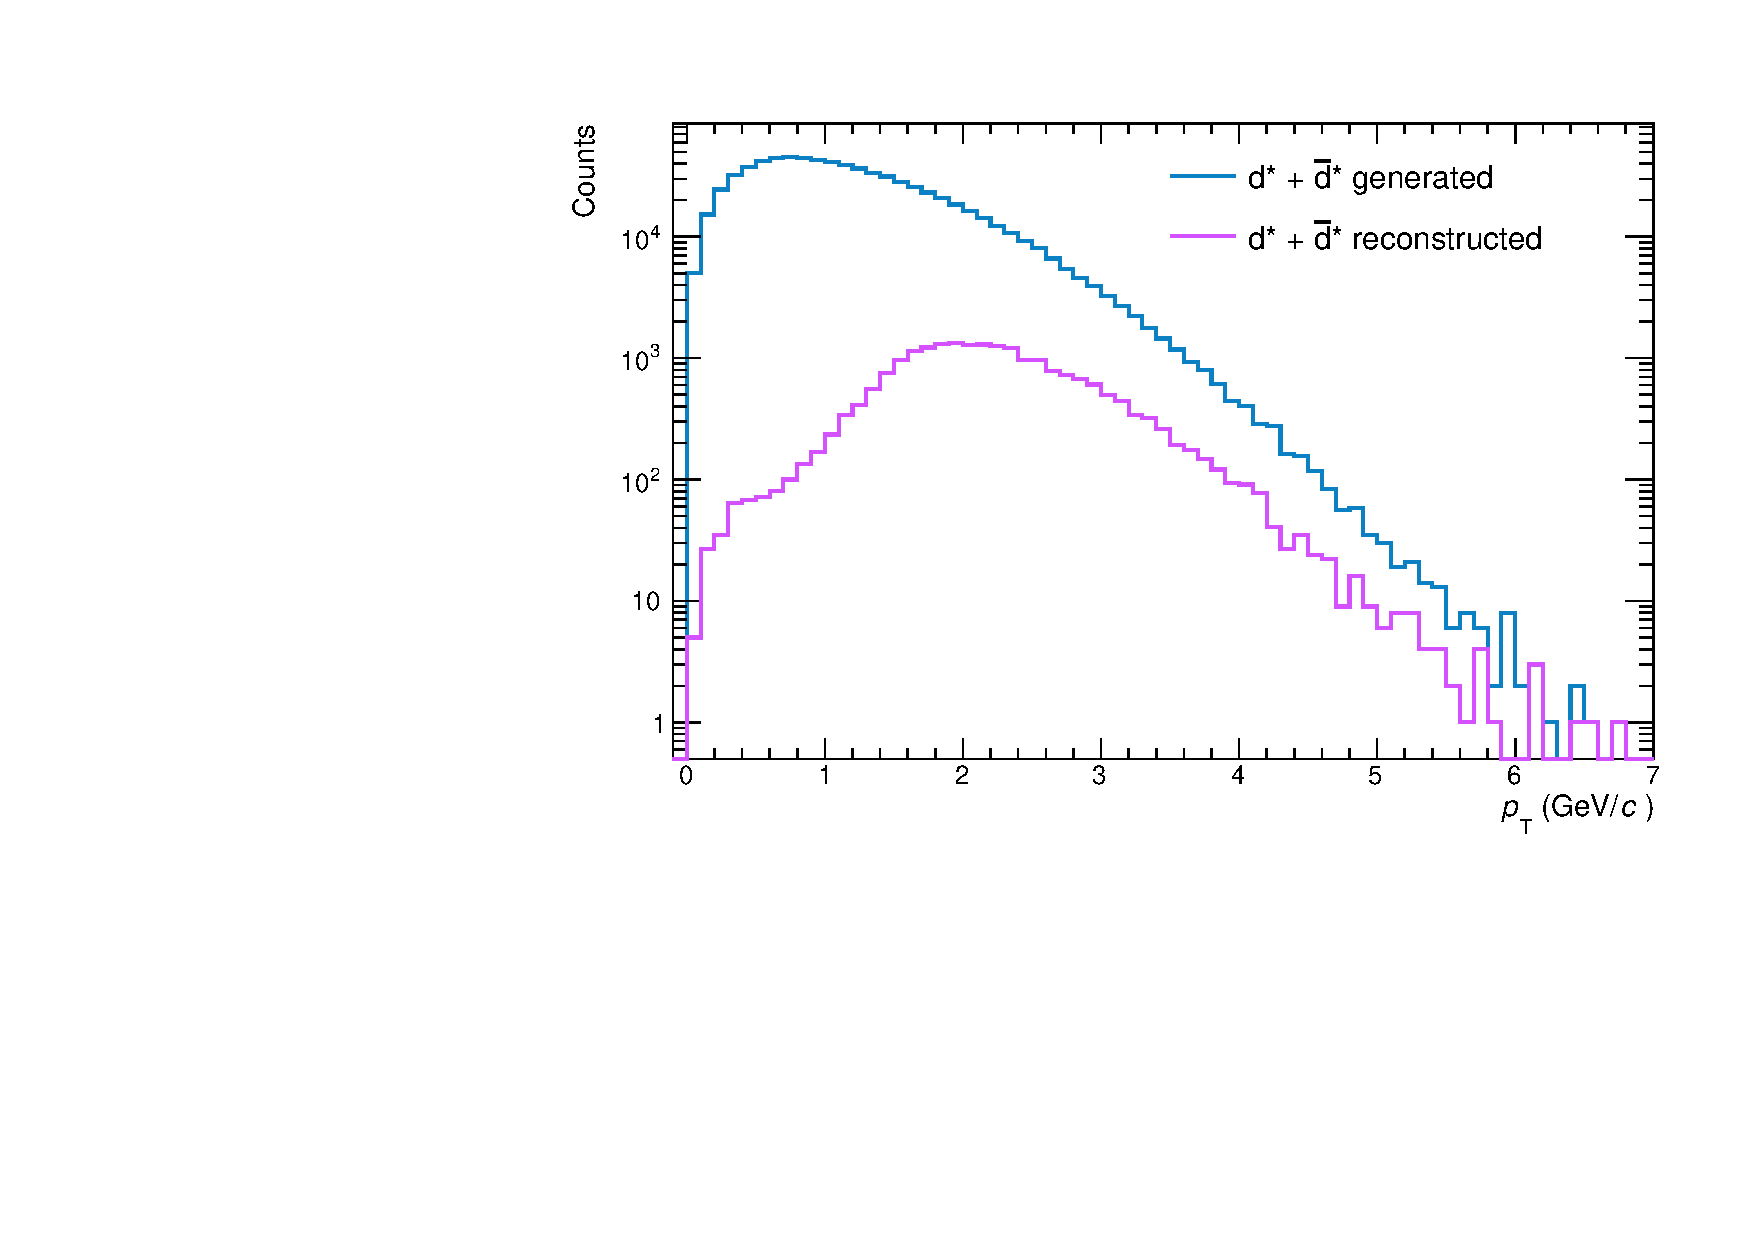
\includegraphics[width=0.5\textwidth]{gfx/genrecBW}
	\caption{Spectrum for both generated (blue line) and reconstructed (magenta line) \ds obtained with Blast Wave rejection sampling.}
	\label{fig:bw_spectrum}
\end{figure}

\begin{figure}
\begin{subfigure}{.5\textwidth}
  \centering
  \captionsetup{justification=centering}
  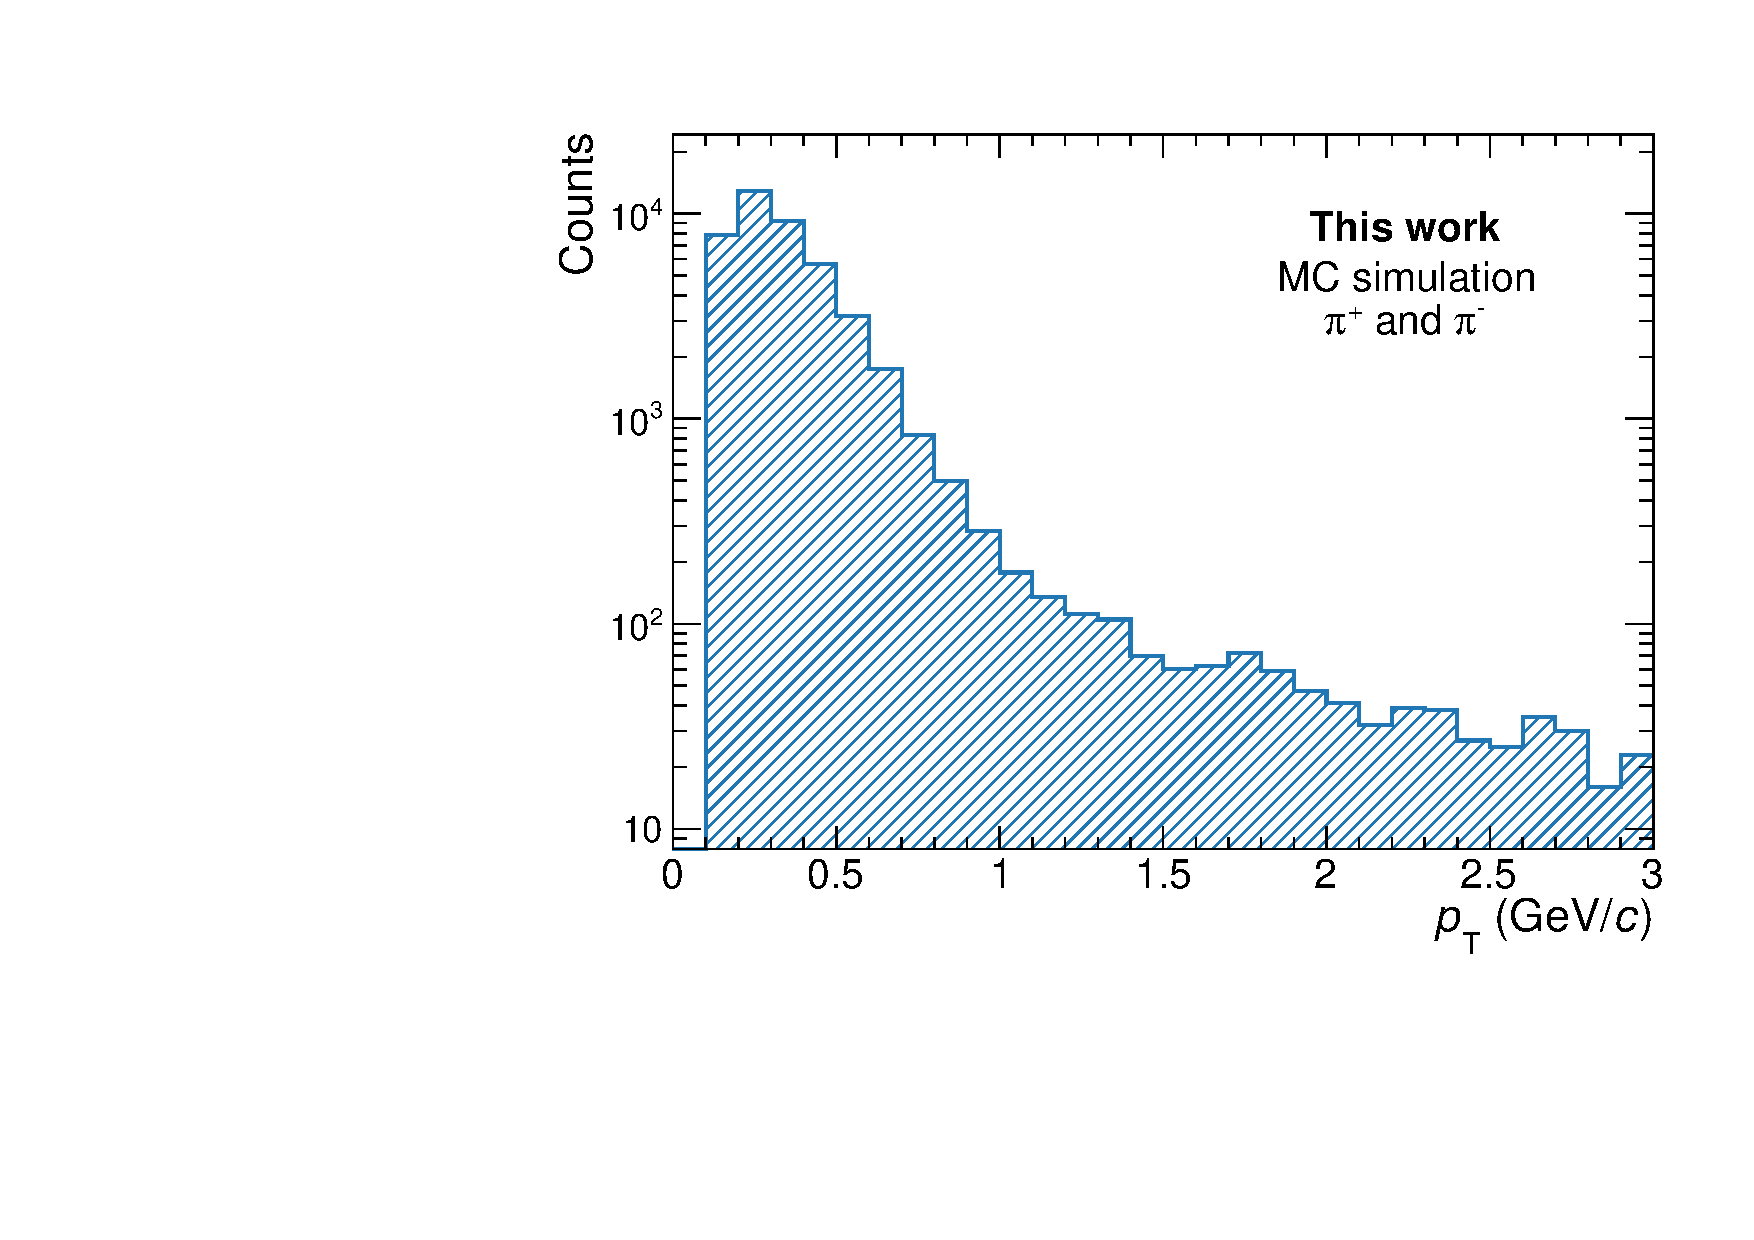
\includegraphics[width=\linewidth]{gfx/pi_spectrum}
  \caption{}
  \label{fig:pi_spectrum}
\end{subfigure}%
\begin{subfigure}{.5\textwidth}
  \centering
  \captionsetup{justification=centering}
  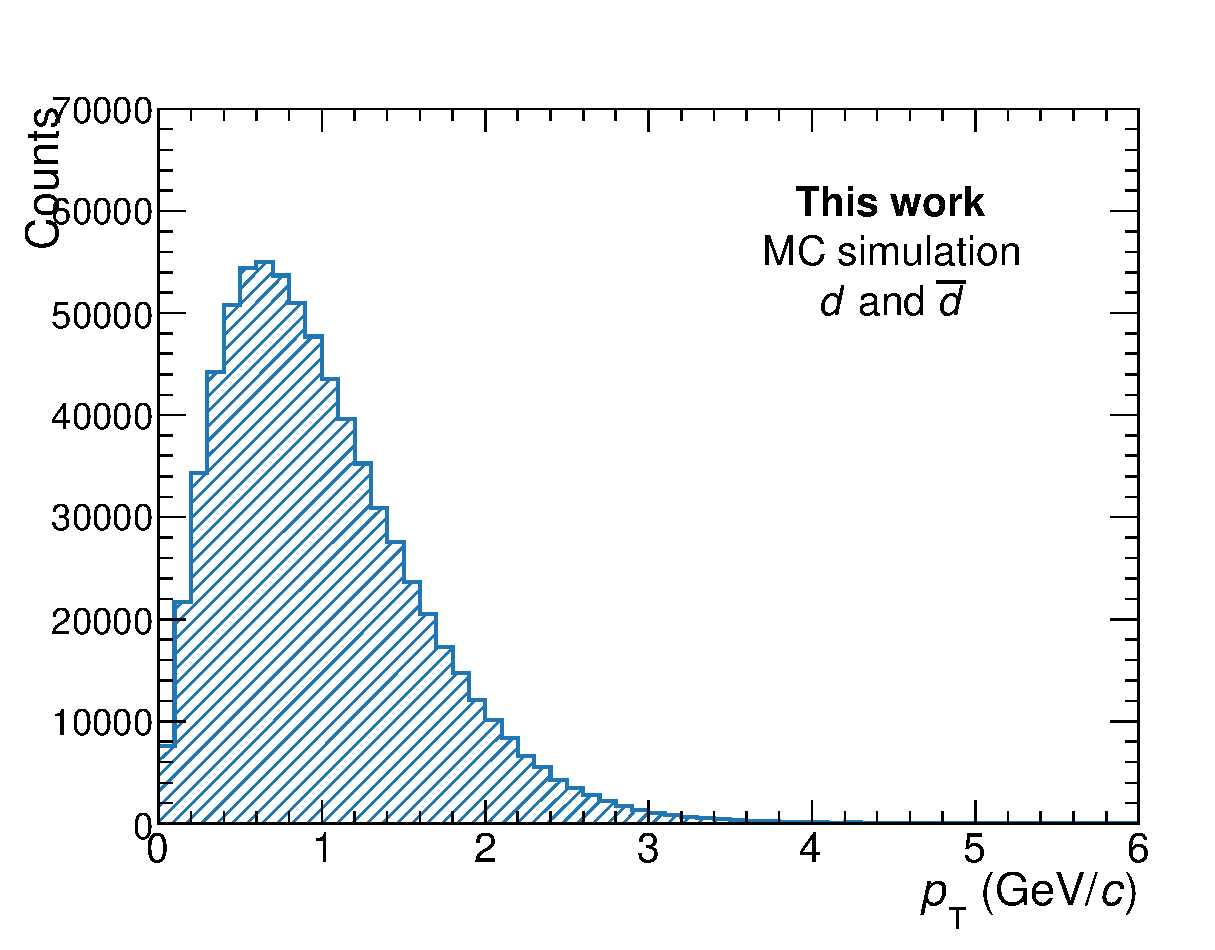
\includegraphics[width=\linewidth]{gfx/deu_spectrum}
  \caption{}
  \label{fig:deu_spectrum}
\end{subfigure}
\caption{Expected transverse momentum spectrum for the \ds decay product derived with the rejection sampling: pions in panel (a) and deuterons in panel (b).}
\label{fig:BW_spec_prod}
\end{figure}

%
%
\section{Reconstruction efficiency of the \ds decay} \label{sec:eff}

One of the fundamental steps of the analysis presented in this thesis is to evaluate if the
\dstdecay is detectable by the ALICE apparatus, considering reconstruction efficiency and acceptance
of the ALICE detectors. 

Furthermore, if the decay is visible, the measured raw yields are biased by inefficiencies in the
ALICE detectors.
For instance, the active area of the experiment is not hermetic by design or, sometimes, parts of
the detectors might be switched off during some data taking periods due to technical problems,
reducing the efficiency.
The acceptance, instead, is only related to the geometric coverage of the detectors.

It is possible to correct for the finite efficiency and acceptance using a MC simulation where the
full geometry and the real data taking conditions are reproduced. The MC production used for this
analysis has been described in Section \ref{sec:4.2}. 
The number of particles crossing the detectors and their kinematics observables are known when using
the MC simulation and the efficiency$\times$acceptance can be computed as:
\begin{equation}
    Efficiency \times Acceptance\ (\pt) = \frac{\mathrm{N}_{\textit{rec}}(\pt)}
    {\mathrm{N}_{\textit{gen}}(\pt)},
\end{equation}
where $\mathrm{N}_{\textit{gen}}$ is the number (\dsbar)\ds generated in the azimuthal region
$0 \leq \phi < 2\pi$ and in the $|y| < 0.5$, while $\mathrm{N}_{\textit{rec}}$ is the number of 
(\dsbar)\ds for which the decay products satisfies the selection criteria described in Section
\ref{sec:track_sel_crit}.

Since anti-deuterons can be absorbed by detectors material, the efficiency for \dsbar is
expected to be lower than \ds.
Therefore the efficiency $\times$ acceptance is evaluated for \ds and \dsbar separately as a
function of the transverse momentum for the three PID configurations. 
The results are shown in Figure ~\ref{fig:effAM}.

The TPC only configuration has the highest efficiency,
but in the light of the considerations of Section ~\ref{sec:ds_candidate} has also a high 
contamination of the deuteron sample.
The TPC-TOF configuration has a very low efficiency, due to the high pions suppression 
resulted from the use of TOF for their identification. 
Instead the TPC+TOF$_{deuteron}$ configuration guarantees a good efficiency and should also ensures
a better deuteron sample purity than the TPC configuration.

\begin{figure}
    \centering
    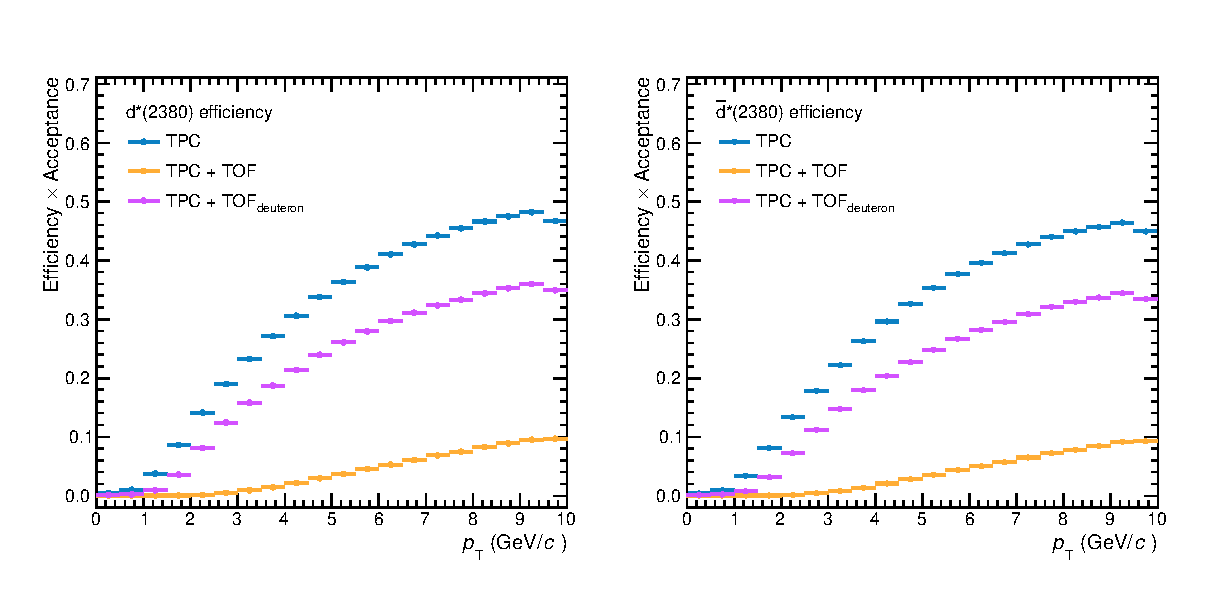
\includegraphics[width=\textwidth]{gfx/eff3globalSLIM}
	\caption{Reconstruction efficiency of the \ds (left panel) and \dsbar (right panel) decay as a function of the transverse momentum for the three considered PID configurations.}
	\label{fig:effAM}
\end{figure}

A more accurate evaluation of the discrepancy between \ds and \dsbar efficiency has been done
by computing the \ds/\dsbar efficiency ratios for all the PID configurations.
In Figure ~\ref{fig:eff_ratioAM} the ratio computed for TPC+TOF$_{deuteron}$ is reported.

\begin{figure} [!h]
    \centering
    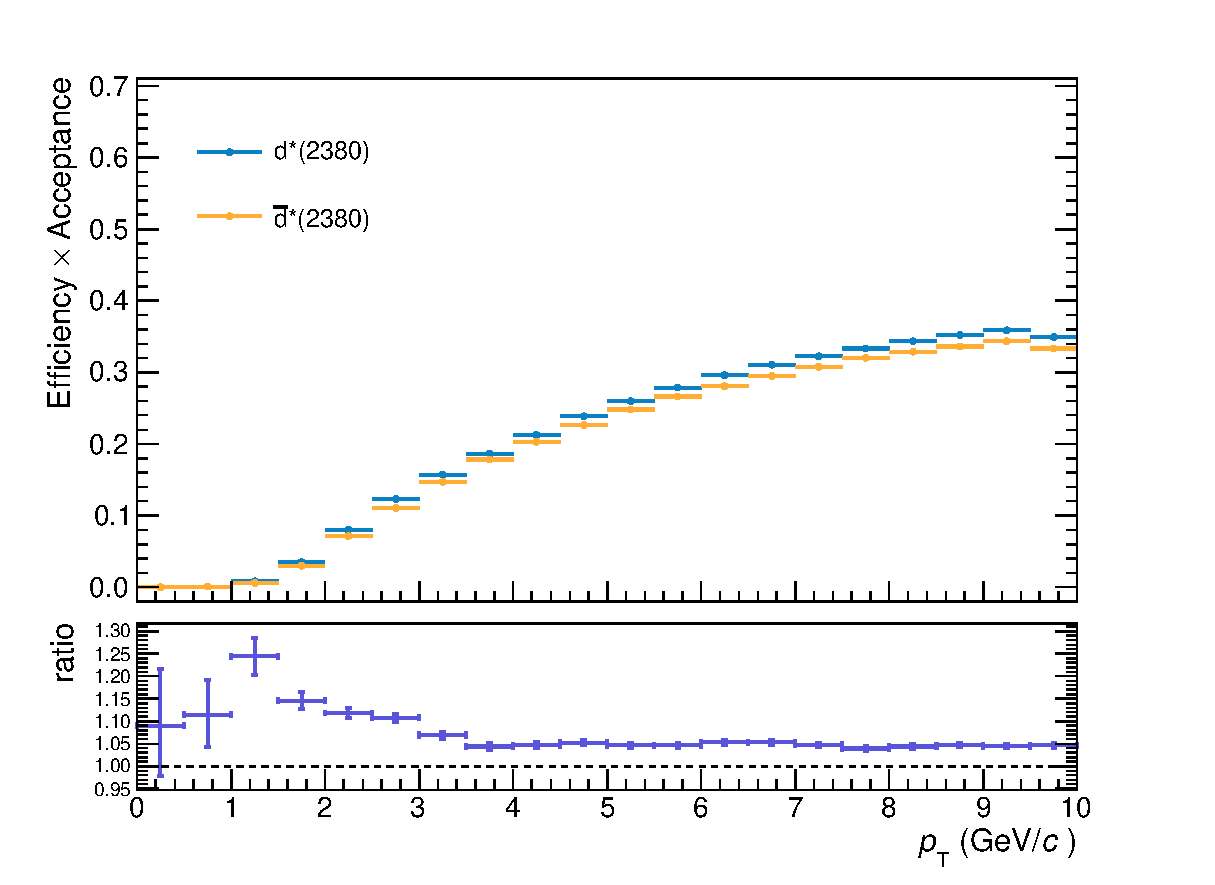
\includegraphics[width=0.8\textwidth]{gfx/eff_ratioAM1SLIM}
	\caption{The efficiency $\times$ acceptance for both \ds and \dsbar is compared for the TPC+TOF$_{deuteron}$ configuration. The \ds/\dsbar efficiency ratio is also reported and shows a behaviour compatible with what expected from the anti-deuteron cross section with material.}
	\label{fig:eff_ratioAM}
\end{figure}

The relative difference between \ds and \dsbar efficiency is higher than $15$ \% for 
$\pt < 3\;\gevc$, instead at higher \pt is $\sim 6\ $\%. 
These values are compatible with what is expected from the anti-deuteron cross section with material,
that decreases at higher \pt.

The determination of which the PID configuration shall be chosen,
must be made considering the momentum region in which the \ds is expected to be produced more 
abundantly.
In the light of the study of the expected \ds momentum spectrum (Sec. ~\ref{sec:spectrum}), the 
crucial region for the efficiency is the $0 - 2\;\gevc$ \pt interval.
Therefore the TPC/TPC+TOF$_{deuteron}$ efficiency ratio has been computed and compared with the expected
\ds transverse momentum spectrum.
The Figure ~\ref{fig:eff_spec} shows the comparison between this two configurations and the expected \pt
spectrum of the \ds.

\begin{figure}
    \centering
    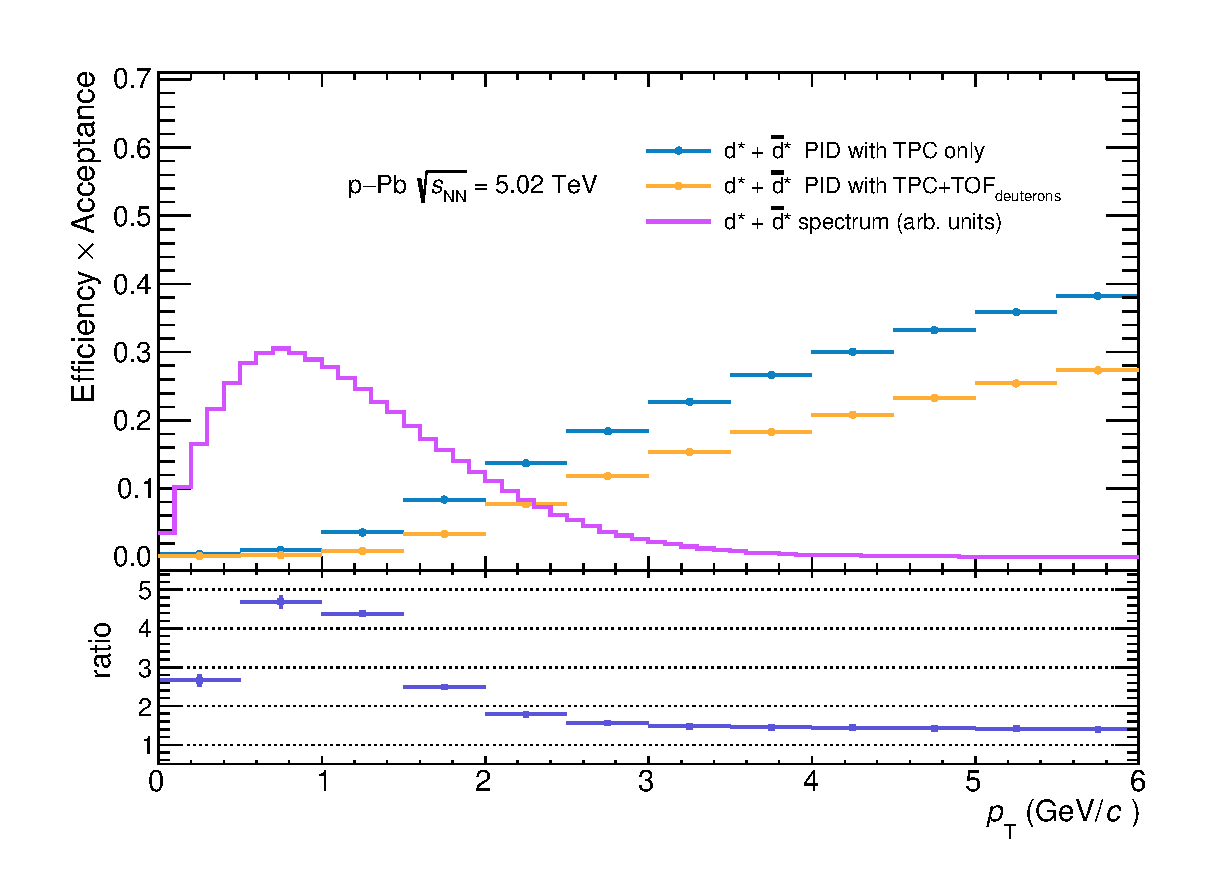
\includegraphics[width=0.8\textwidth]{gfx/effspecSLIM}
	\caption{The expected \pt distribution for the \ds derived in Section ~\ref{sec:spectrum} is superimposed to the efficiency computed for TPC and TPC+TOF$_{deuteron}$ PID configurations. The ratio between the efficiencies of the two configurations is also reported.}
	\label{fig:eff_spec}
\end{figure}

Both the TPC and TPC+TOF$_{deuteron}$ configurations have low efficiencies ($< 0.02$) in the $0 - 1\;\gevc$
interval. While in the $1 - 2\;\gevc$ interval the TPC configuration efficiency reach the value of 0.10.
In the whole $0 - 2\;\gevc$ interval the TPC efficiency is 3-5 times higher than the TPC+TOF$_{deuteron}$.


Nevertheless, the choice of which PID configuration should be used is still not trivial. 
In order to observe the \ds signal is crucial to have a good signal/background ratio that depends
both from the efficiency and the purity of considered sample.
The usage of the TOF for the identification of the deuteron ensure a reduced contamination \ -- from 
other particle species -- \ of the deuteron sample. 
Therefore the TPC+TOF$_{deuteron}$ configuration could have better performance in terms of the 
signal/background ratio, respect to the TPC configuration.

%
%
\section{Study of the background of the measurement} \label{sec:background}

In order to perform the background subtraction described in Section ~\ref{sec:4.1} is necessary to have
a model that satisfactorily reproduce the background of the measurement. 
Therefore two different background models has been developed and tested. 
In this section the models and their performances in describing the background will be discussed.

In this work the main difficulty is to manage to describe and reproduce the backgrounds due to pions.
In fact, in \pPb collisions many particle species are produced \cite{pkp_prod, neutralp, k0s_prod} 
and most of them have a decay channel that include a charged pion.
In particular neutral mesons, e.g. $\eta,\,\omega,\,K_{s}^{0}$ mesons, have a 
\pip + \pim decay channel. Other pions, as well as deuterons, can be produced directly
in the hadronization phase of the collision.
All of these pions and deuterons contribute to the background of the measurement of the
\dstdecay decay. In fact one can make a \textit{\ds candidate} (Sec. ~\ref{sec:ds_candidate})
matching this particles not originating from a real \ds decay.

The two models are both based on the event mixing technique.
event mixing, basically, is a method used to reproduce uncorrelated background combining particles from
different events, this ensures that there can’t be correlation between considered particles.
This technique can be very effective, but it is necessary to be careful in mixing particles from 
similar events.
So it is very important to mix particles from events with comparable vertex and particle multiplicity 
and to study the performance of this method with different classifications of similar events.
event mixing can be very expensive in terms of memory usage, because it is necessary to store in memory
lots of events that will later be combined with others.
The tool used to store events has been specifically developed for providing an efficient memory usage.
Different events classifications were studied for both models, in order to find the setup that 
guarantees the best background description.




Having lots of pions per event

The two models developed to describe the \dsdecay background are based on different approaches to the
problem.





For the measurement of the \dstdecay the main sources of backgrounds are the pions. 

%
\subsection{Partial Event Mixing model} \label{sec:pem}

The partial event mixing model (PEM) tries to reproduce both correlated and uncorrelated backgrounds
combining between them pion pairs from the same event with deuterons from another.
In principle this ensure to break the correlation between \textit{\ds candidates} because not all three
particles are taken from the same event.
At the same time, it should correctly describe the correlations between pions because they are taken from the 
same event.
Events are classified by the position of the vertex along the $z$ axis ($z_{vertex}$) only. Classification 
by particle multiplicity of the event was tested, but has not been used because it’s not effective.
Different $z_{vertex}$ classifications has been studied, the final choice is a $10\ $ class of $1\;$ cm
classification in the $-10 < z_{vertex} < 10$ cm interval.

For each event, every pion pairs is combined with 5 different deuterons from 5 different events
with $z_{vertex}$ in the same class.
The model is compared with the \minv distribution \ -- outside the region of interest -- \ in 3
different intervals of the transverse momentum of the \textit{\ds candidates}:
\begin{itemize}
    \item 0 -- 1 \ \gevc
    \item 1 -- 2 \ \gevc
    \item 2 -- 3 \ \gevc
\end{itemize}
Since the \ds production is expected to be negligible for $\pt > 3$ \gevc the comparison between the
model and the \minv has been performed only in this intervals.

\begin{figure}
\begin{subfigure}{.33\textwidth}
  \centering
  \captionsetup{justification=centering}
  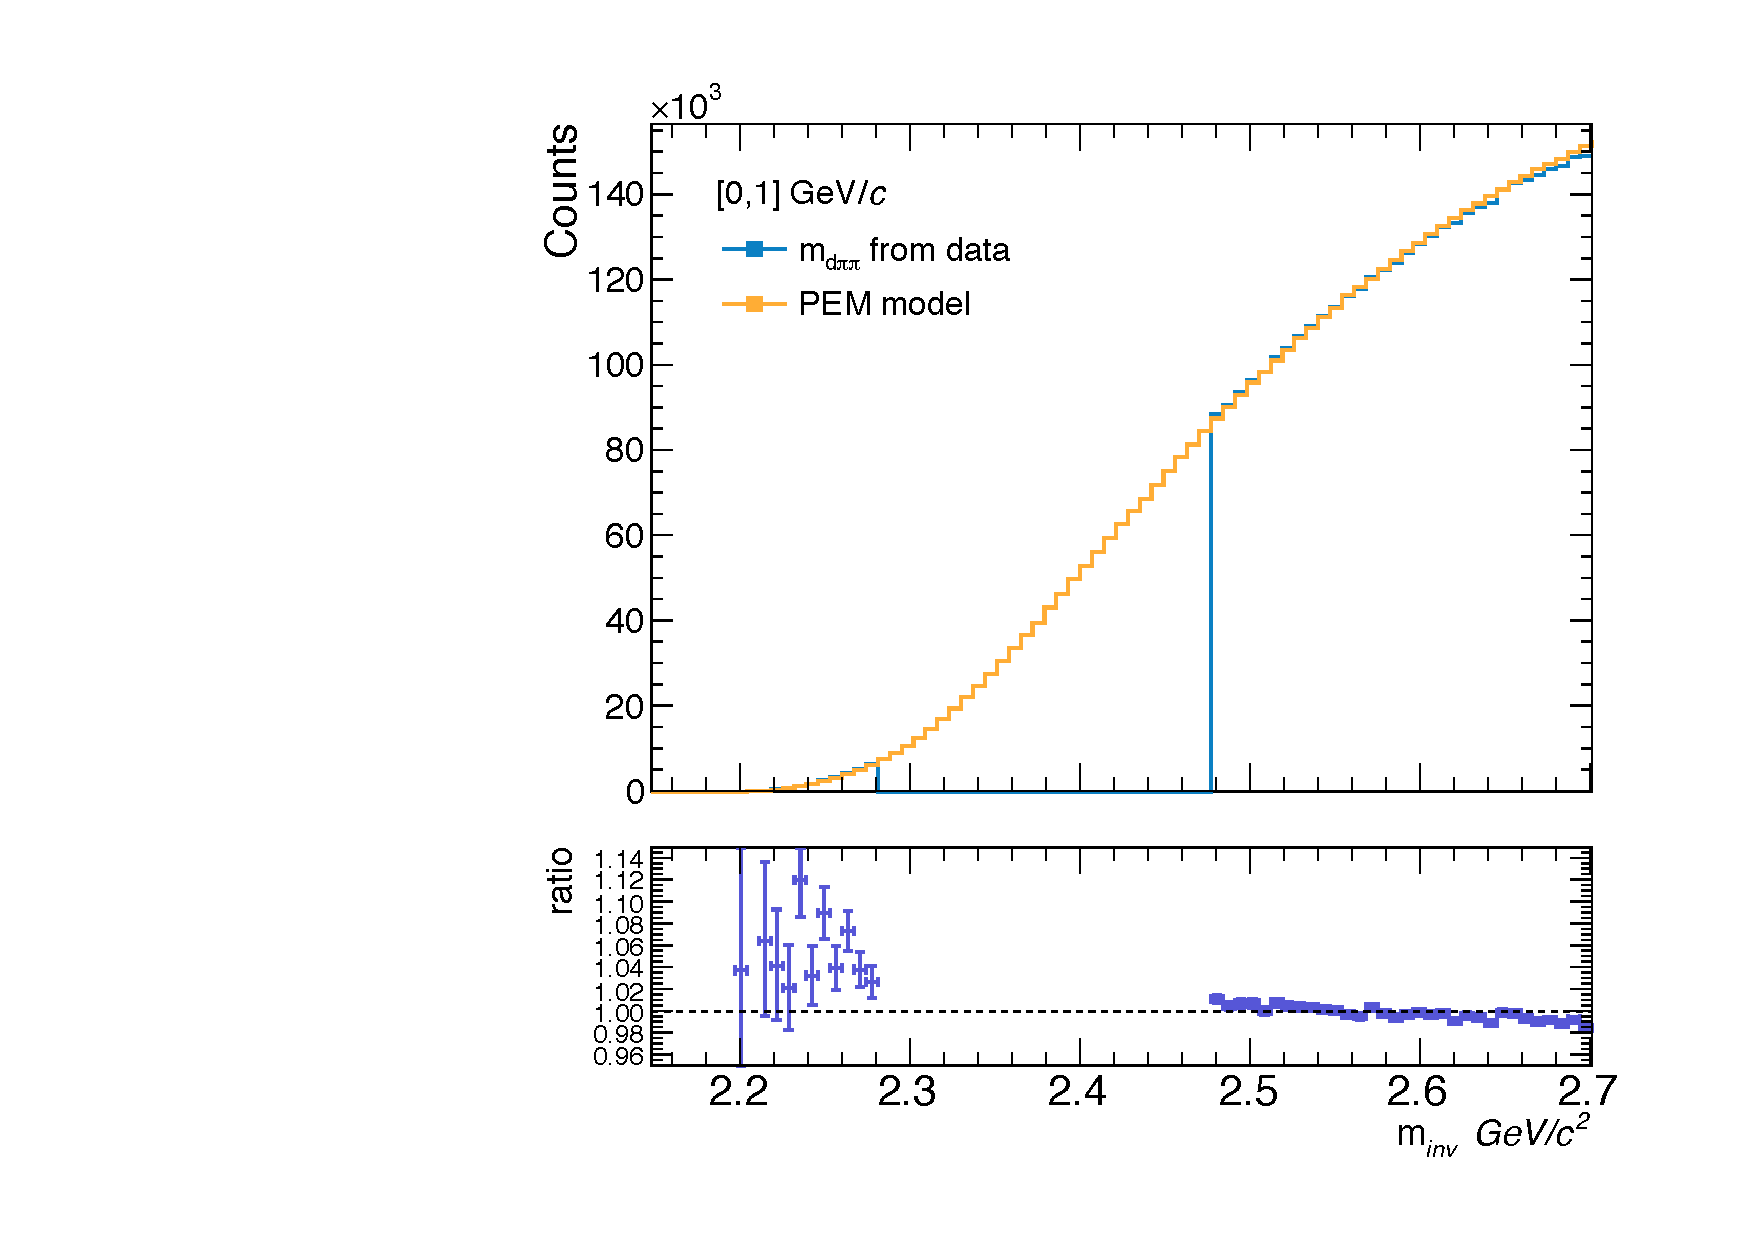
\includegraphics[width=\linewidth]{gfx/01}
  \caption{}
  \label{fig:pem01}
\end{subfigure}%
\begin{subfigure}{.33\textwidth}
  \centering
  \captionsetup{justification=centering}
  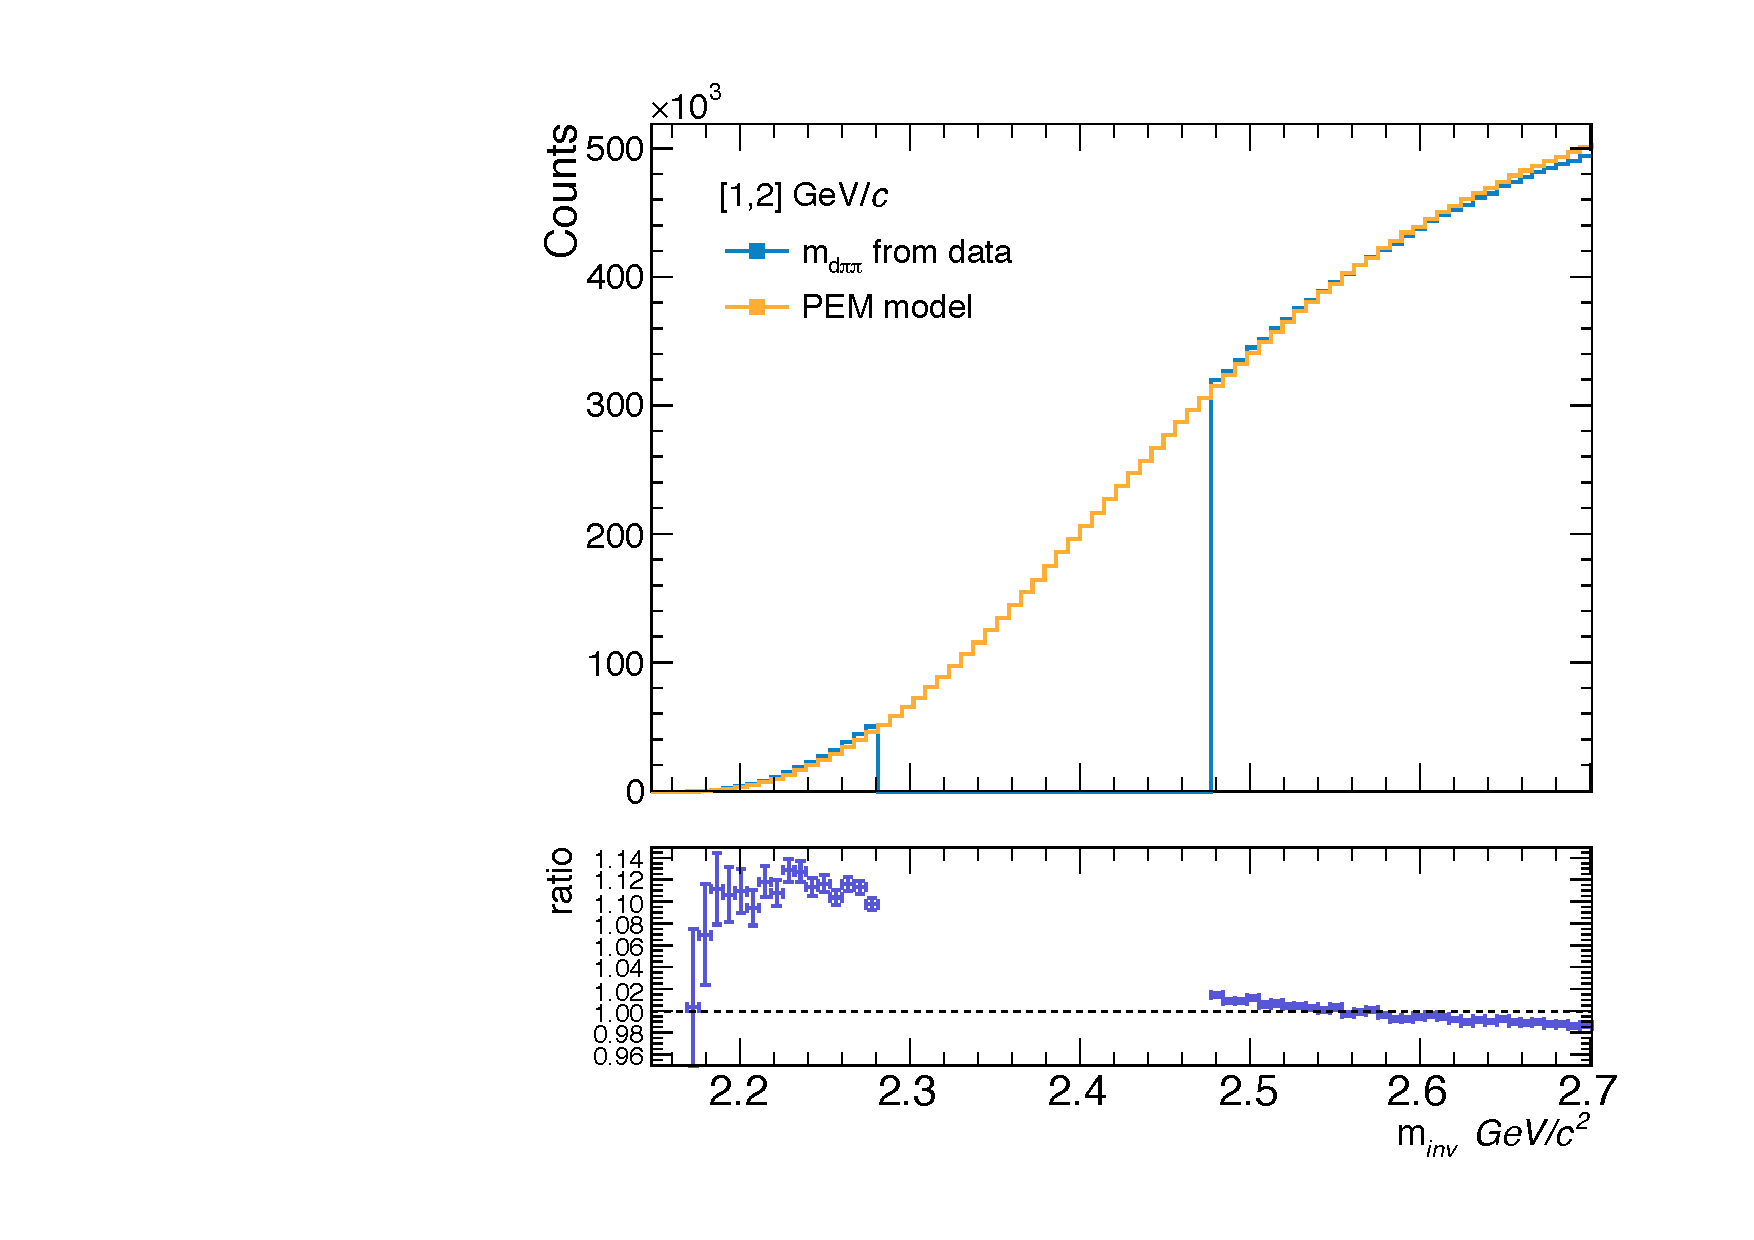
\includegraphics[width=\linewidth]{gfx/12}
  \caption{}
  \label{fig:pem12}
\end{subfigure}
\begin{subfigure}{.33\textwidth}
  \centering
  \captionsetup{justification=centering}
  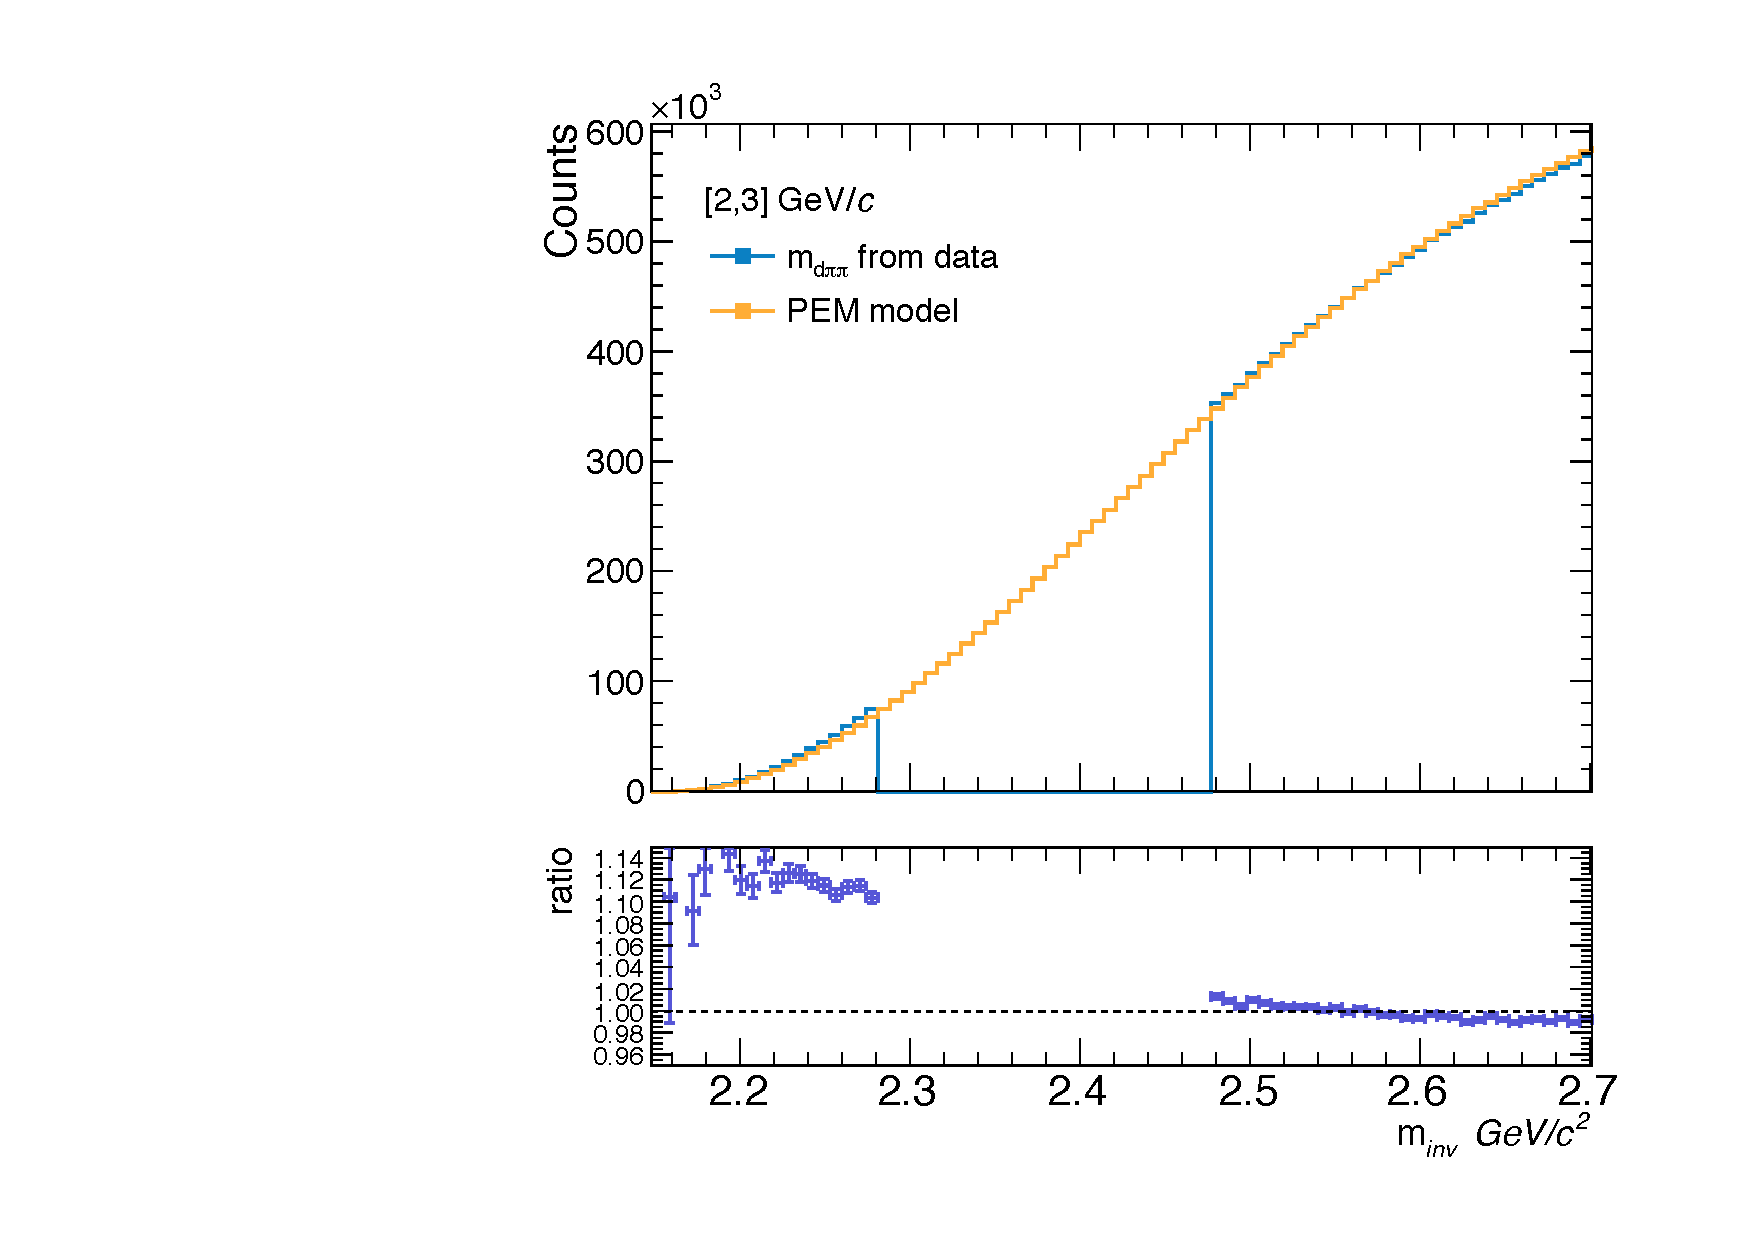
\includegraphics[width=\linewidth]{gfx/23}
  \caption{}
  \label{fig:pem23}
\end{subfigure}
\caption{PEM model compared with \minv in the three considered \pt intervals.}
\label{fig:PEM}
\end{figure}
%plot da fare più grandi??

The normalisation of the PEM model to the data has been done in the interval from 2.480 to
2.620 \gevcs. Smaller intervals have been studied, but the final findings do not
change in any meaningful way. The normalisation has not been performed in the region on the left 
of RoI because the model does not well describe the data in that region.

The PEM model can reproduce quite well the data in the region on the right of the RoI,
particularly in the 0 -- 1 \gevc \pt bin (Fig. ~\ref{fig:pem01}). In this region the difference between
data and model is < 2\%, but a trend is clearly visible in the ratio.
This trend is bigger in 1 -- 2 \gevc and 2 -- 3 \gevc \pt bins (Figure ~\ref{fig:pem12}, 
~\ref{fig:pem23} respectively).
Instead the left sideband is not reproduced by this model in all three \pt bins.

The background description provided by the PEM model is not satisfactory in the whole \pt range
considered. One can think that the discrepancies from data are due to some deuteron-pion correlation
that we are not considering.

Therefore another component of the PEM model has been derived mixing $d-\pi$ pairs from the
same event and other pion from another event.
The resulting model is the weighted sum of the $\pi-\pi$ PEM with the $d-\pi$ PEM. 
The relative weight of the 2 contribution was found fitting the model to the data outside the RoI
with the relative weight as fit parameter.
This new model improves the background description.
In the first two \pt bin the data/model ratio is almost the same as in the case of the previous model,
while in the last one (Fig. ~\ref{fig:pem_imp23}) the discrepancies in the left sideband are < 3\%.
This value, compared with the previous 12\% of discrepancies shows that the new PEM
model provides a better background description.

\begin{figure}
\begin{subfigure}{.33\textwidth}
  \centering
  \captionsetup{justification=centering}
  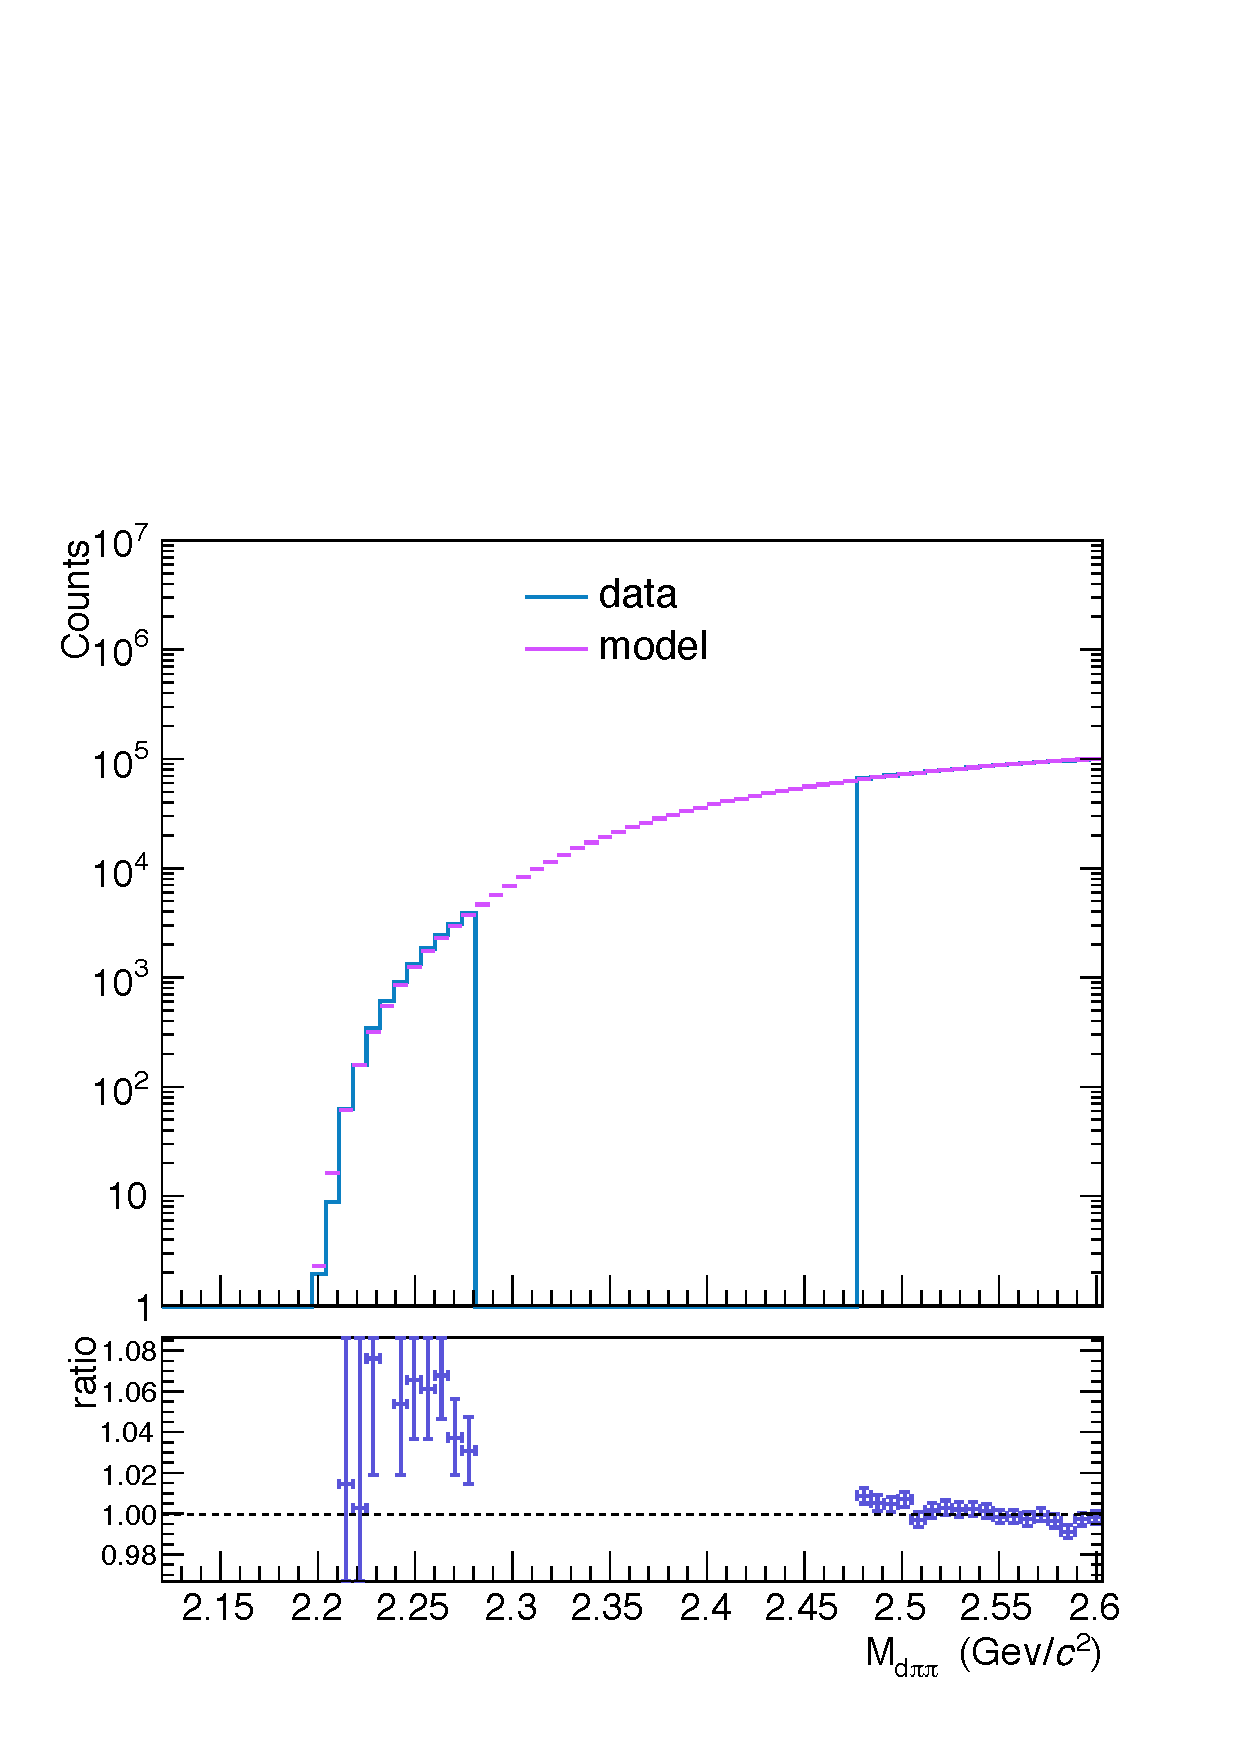
\includegraphics[width=\linewidth]{gfx/PEMimp0}
  \caption{}
  \label{fig:pem_imp01}
\end{subfigure}%
\begin{subfigure}{.33\textwidth}
  \centering
  \captionsetup{justification=centering}
  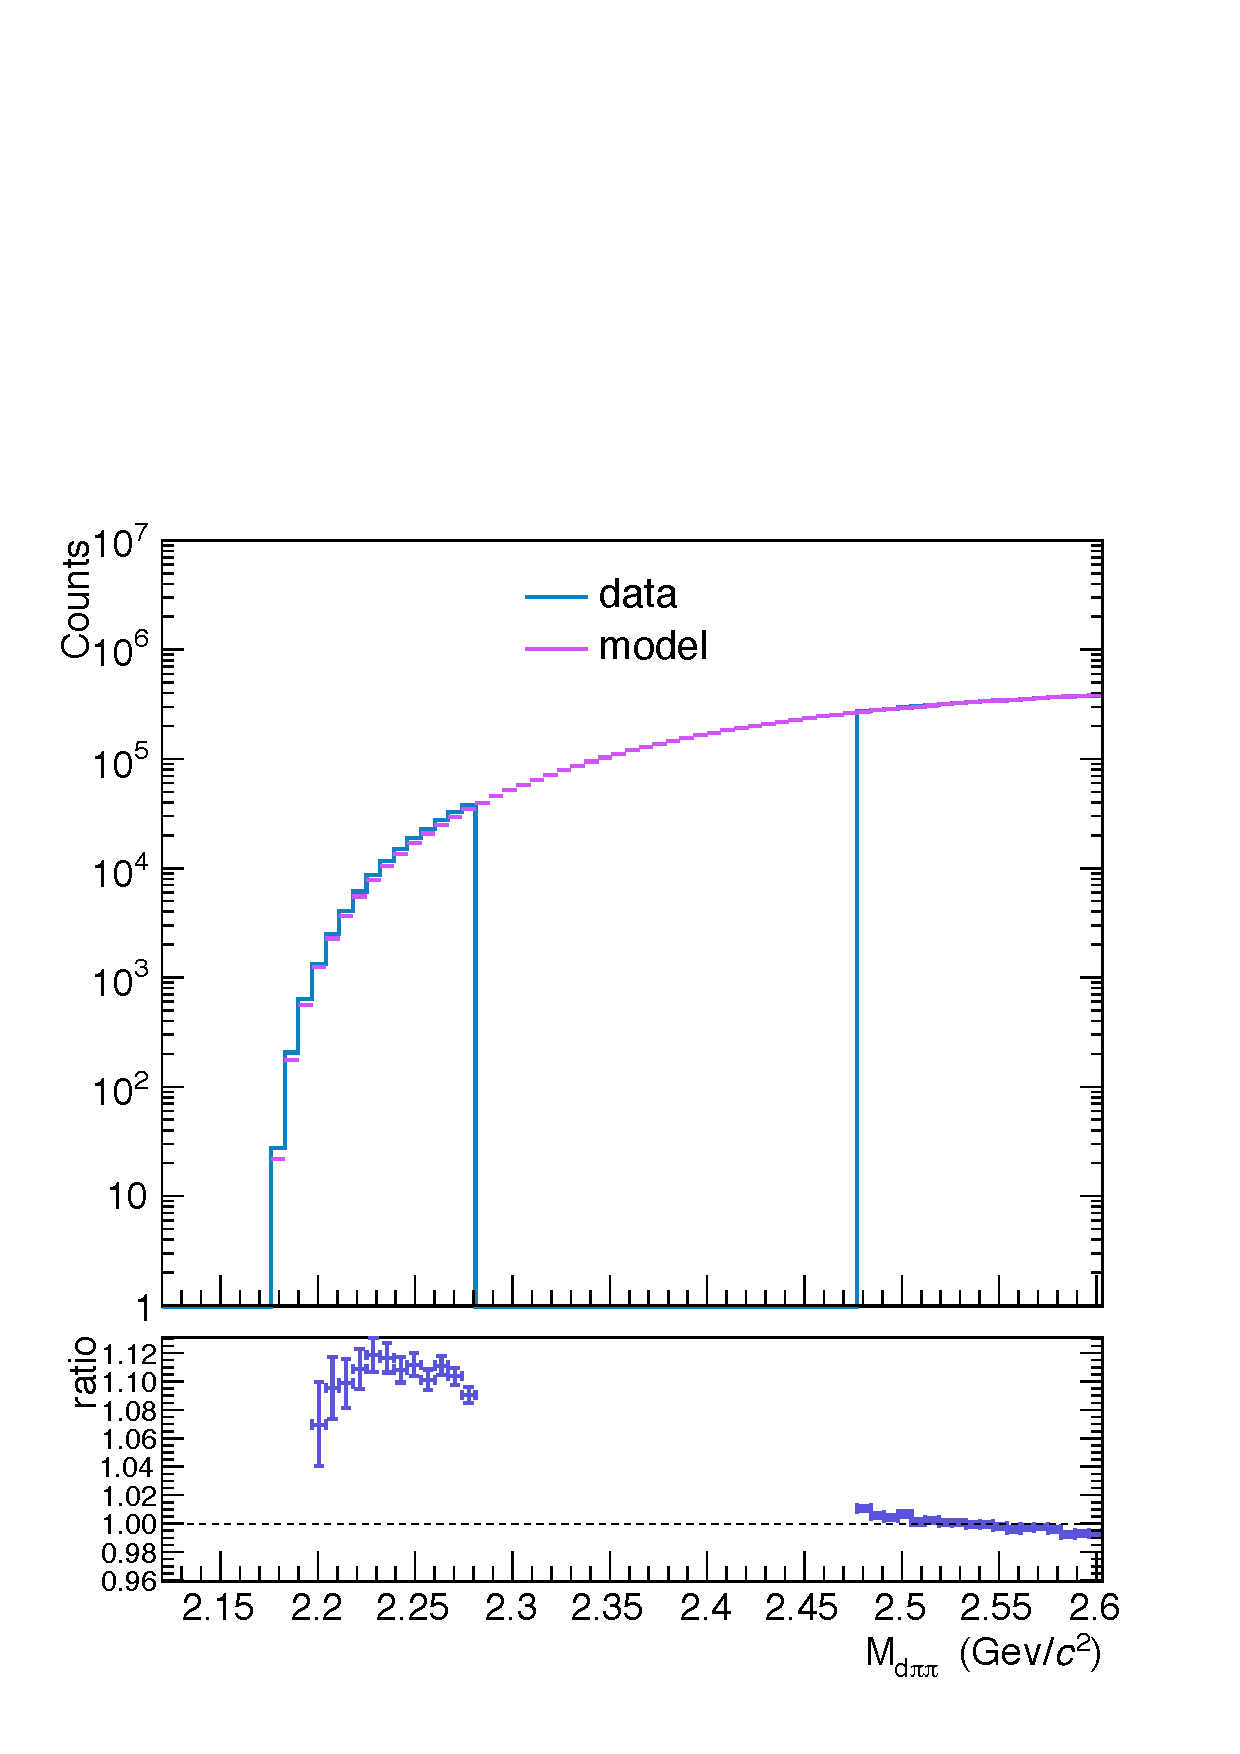
\includegraphics[width=\linewidth]{gfx/PEMimp1}
  \caption{}
  \label{fig:pem_imp12}
\end{subfigure}
\begin{subfigure}{.33\textwidth}
  \centering
  \captionsetup{justification=centering}
  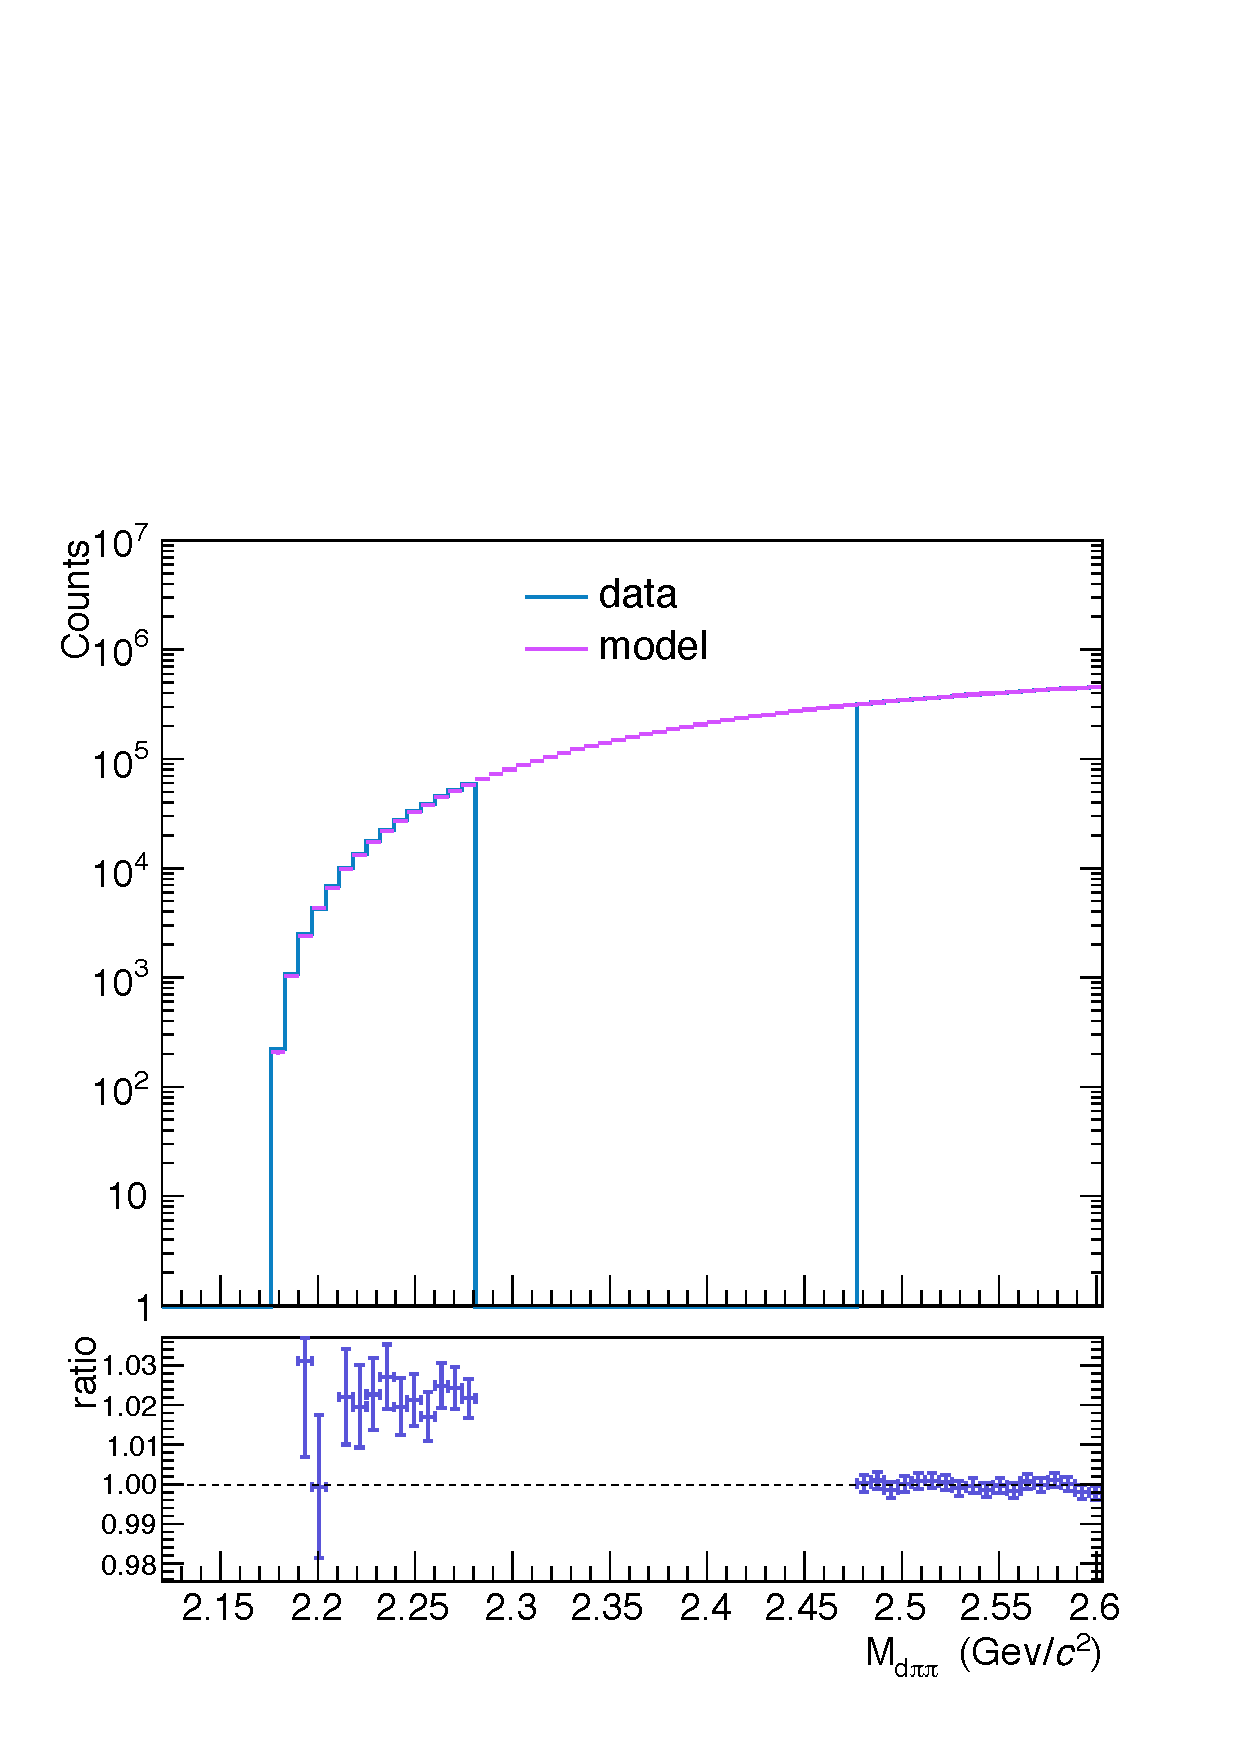
\includegraphics[width=\linewidth]{gfx/PEMimp2}
  \caption{}
  \label{fig:pem_imp23}
\end{subfigure}
\caption{PEM model improved with the $d-\pi$ component compared with \minv in the three considered \pt intervals.}
\label{fig:PEMimp}
\end{figure}

%
\subsection{Template + Event Mixing model} \label{sec:tem}

The Template + Evnt Mixing model tries to reproduce the correlated backgrounds with a Monte Carlo based template
for each background component, while the uncorrelated background is described with a real classical event mixing
with all three tracks from three different events.

The templates are obtained combining deuterons from data \ -- to ensure that they have the correct momentum spectrum 
-- \ with pion pairs from Monte Carlo data \ -- in order to have the information about pion mothers.
In the Monte Carlo every reconstructed pion pairs has benn considered.
Looking at the Monte Carlo truth of the pion mothers, the pion sources that provide pion pairs with mass, summed with
deuteron mass, in 2.120 - 2.600 \gevcs range, has been estimated.
Then for each source the template was obtained combining pion pairs \ -- with the same mother imposed -- \ 
with deuterons from the data. 
Basically each template is a \minv histogram with pion pairs from MC \ -- from the same mother and from the same source -- \ 
and deuterons from data. 
Each pion pairs was mixed with 50 different deuterons in the same $z_{vertex}$ class in order to increase the statistics
of the templates.

This process has been done for the three \pt intervals considered, obtaining different templates in each \pt bin.
The remaining background, which should be now totally uncorrelated, is described with a real event mixing, obtained 
combining all three tracks from data from three different events in the same $z_{vertex}$ class.
Templates have been derived for sources with a contribution to the background at least of $10^{-4}$ of the total in each 
\pt bin:
\begin{itemize}
  \item[] 0 -- 1 \gevc $\rightarrow \ \omega(782),\ \eta,\ \rm K_{0}^{S},\ \eta^{'}(958),\ \gamma $
  \item[] 1 -- 2 \gevc $\rightarrow \ \omega(782),\ \eta,\ \rm K_{0}^{S},\ \eta^{'}(958),\ \gamma $
  \item[] 2 -- 3 \gevc $\rightarrow \ \omega(782),\ \eta,\ \eta^{'}(958),\ \rm K_{0}^{S},\ \phi(1020),\ \gamma $
\end{itemize}

In each \pt bin the TEM model has been obtained as the weighted sum of the templates and the uncorrelated comonent,
where the weights are the fractions with which each template contributes to the total background.
The weights were estimated starting from the abundance of each background source considered in the MC production.
Of course there is a degree of uncertainty on the MC abundances, therefore the models has been fitted to the data in each
\pt bin with weights as fit parameters. The weights has been constrained to be in $\pm$10\% range of the MC estimated value.

\begin{figure}
\begin{subfigure}{.33\textwidth}
  \centering
  \captionsetup{justification=centering}
  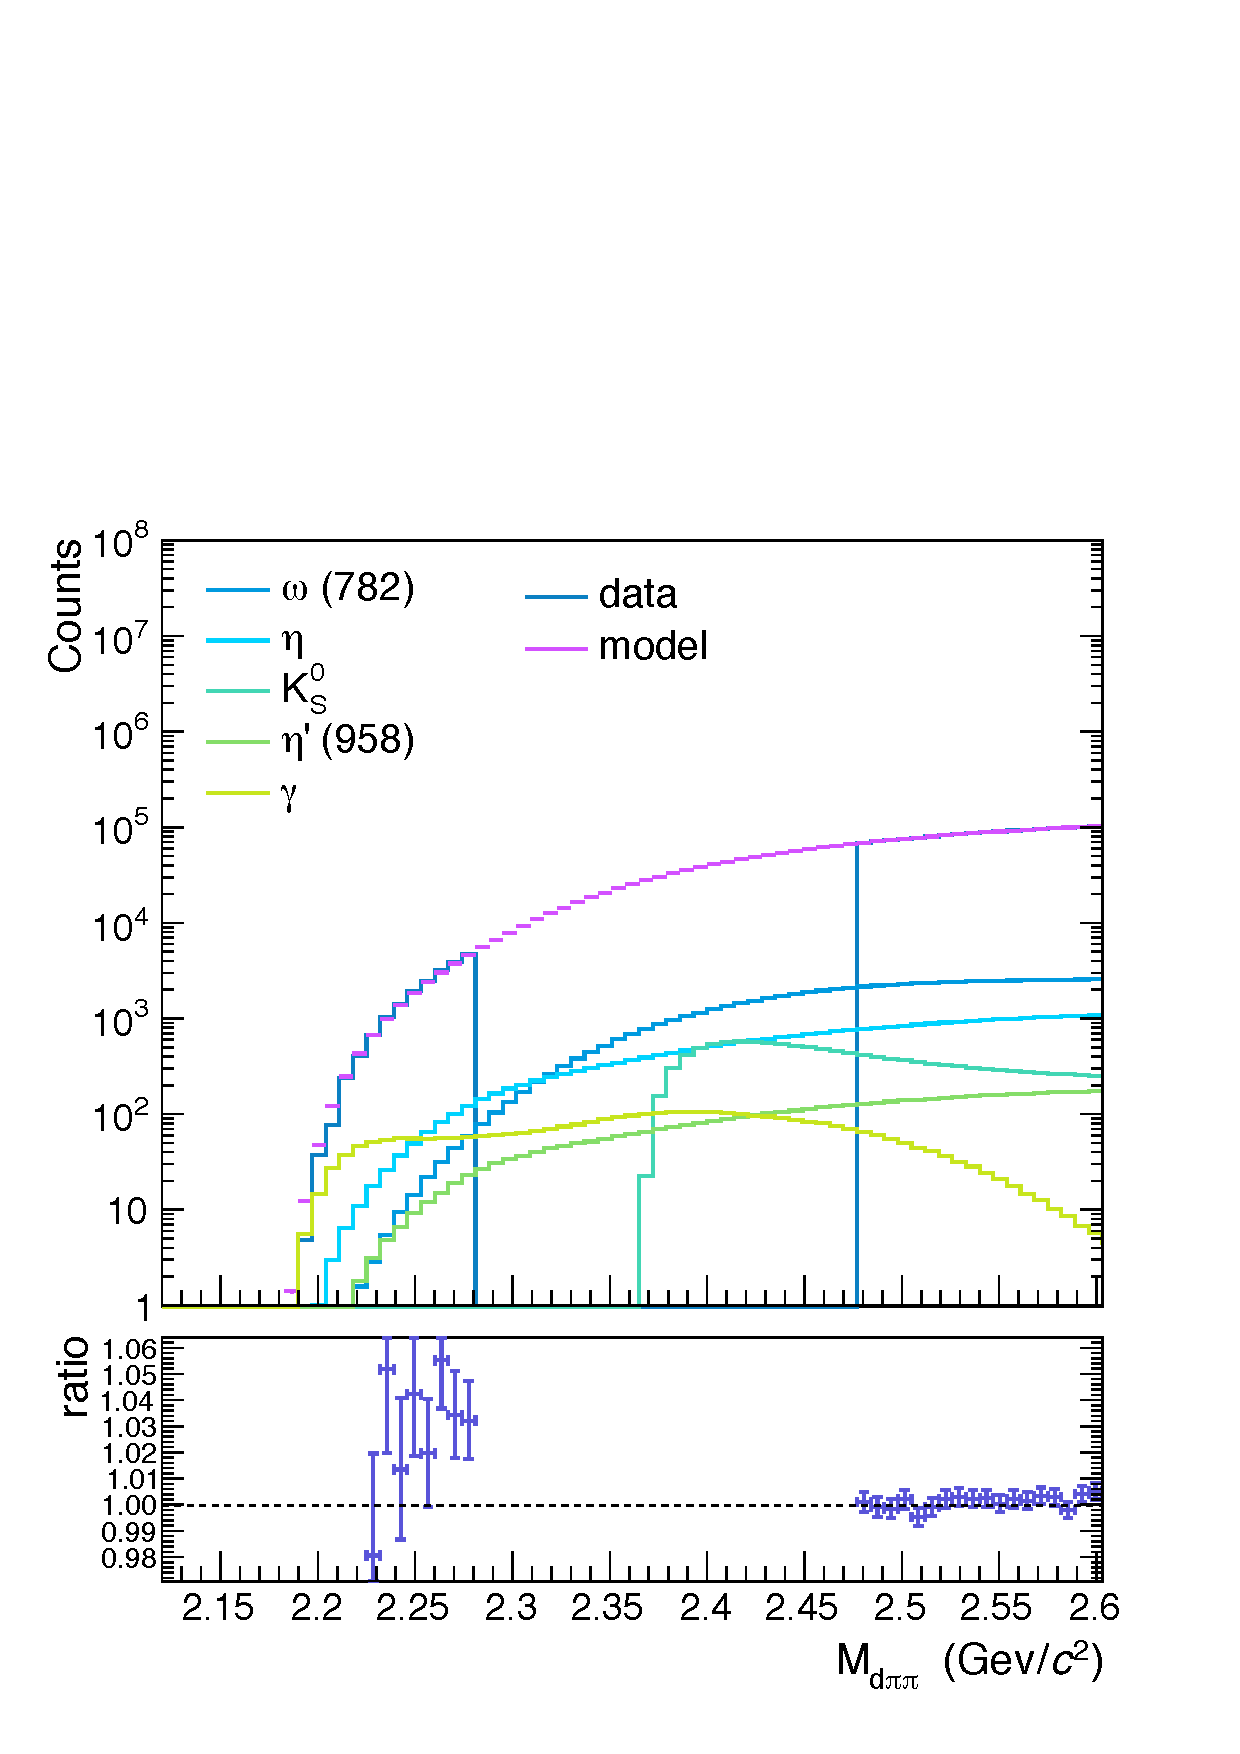
\includegraphics[width=\linewidth]{gfx/can0}
  \caption{}
  \label{fig:tem01}
\end{subfigure}%
\begin{subfigure}{.33\textwidth}
  \centering
  \captionsetup{justification=centering}
  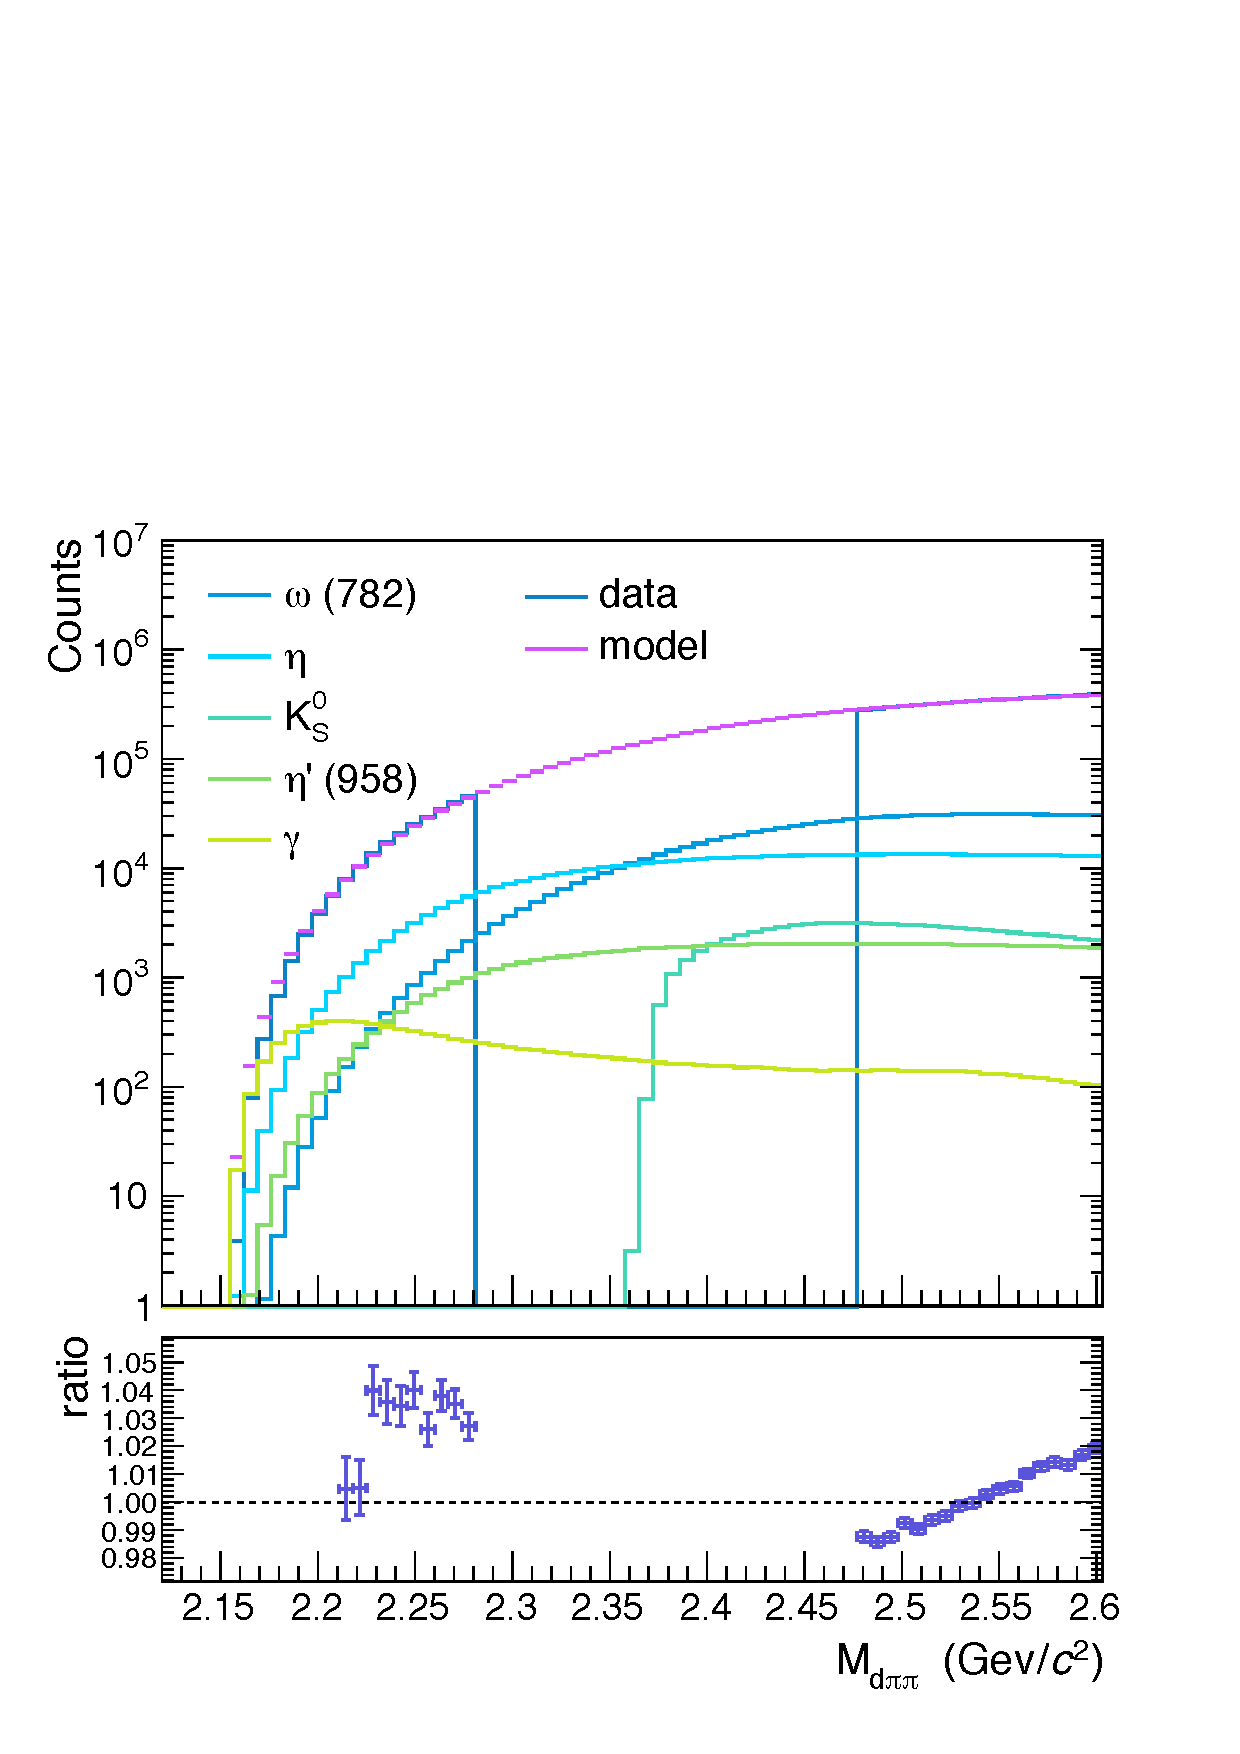
\includegraphics[width=\linewidth]{gfx/can1}
  \caption{}
  \label{fig:tem12}
\end{subfigure}
\begin{subfigure}{.33\textwidth}
  \centering
  \captionsetup{justification=centering}
  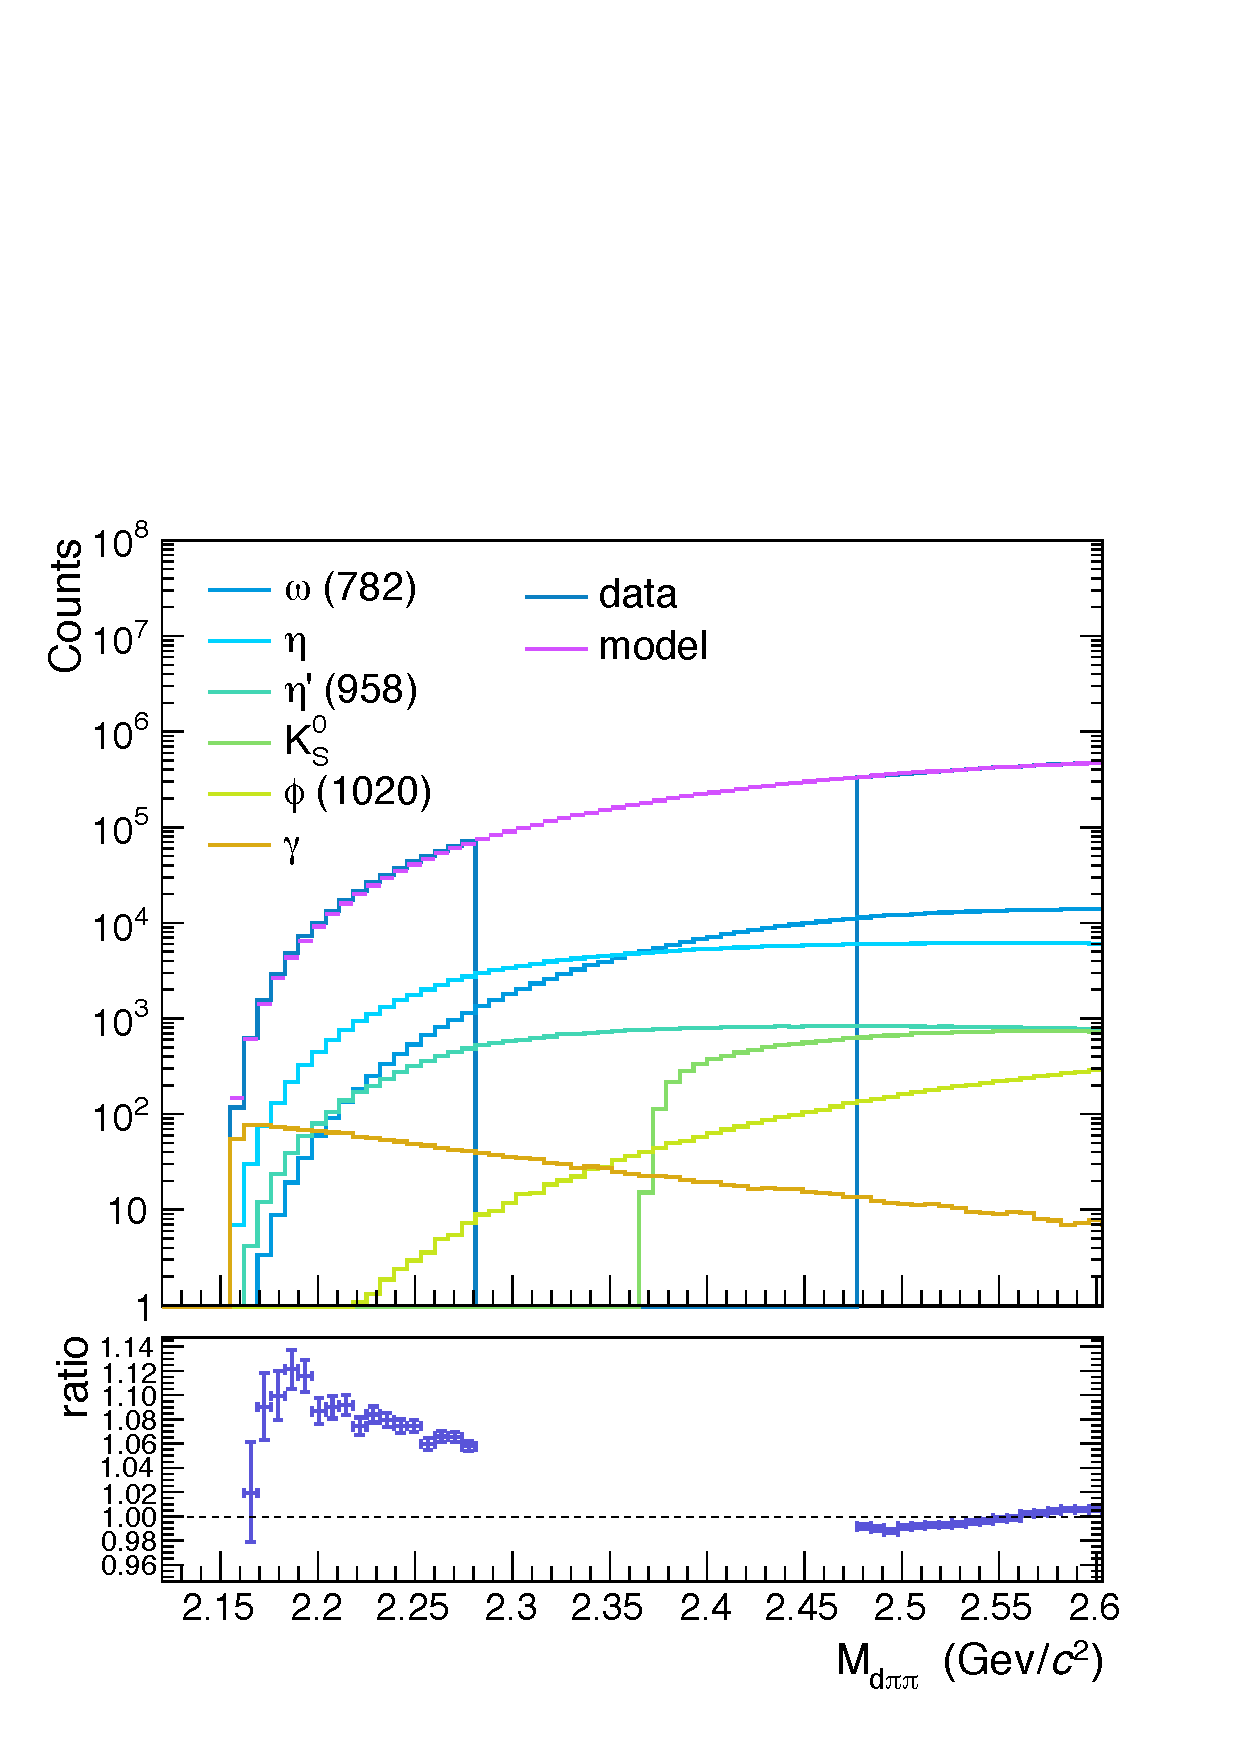
\includegraphics[width=\linewidth]{gfx/can2}
  \caption{}
  \label{fig:tem23}
\end{subfigure}
\caption{The TEM model (magenta line) is compared with \minv from data (blue line) in 0 - 1 \gevc transverse momentum interval. The other lines represent different templates that contribute to the TEM model.}
\label{fig:tem01}
\end{figure}

The TEM model provides a better background description then PEM model. In the first \pt bin
(Fig. ~\ref{fig:tem01}) the data/model ratio is flat in the right sideband, while in the left sideband discrepancies
are around 3\%. In the second bin (Fig. ~\ref{fig:tem12}) the situation is a little worse with a linear trend
in the data/model ratio visible in the right sideband \ -- differences from flat ratio < 2\% -- \ while in
the left sideband the description is similar to that from the first bin. In the last considered bin
(Fig. ~\ref{fig:tem23}) the description get worse, in the right sideband there is a linear trend similar to
the one observed in the second bin, while in the left sideband discrepancies from flat ratio are
around 8−10\%.

The TEM model provides, not only a better background description, but also an estimation of
the background sources and the shapes of their contribution to the total background.

Except for the $K_{s}^{0}$ meson, the templates show a smooth shape, so it is expected that they do not give
rise to suspicious structures in the RoI. The situation is different for the $K_{s}^{0}$ which template has 
the kinematic limit just where the \ds is expected to be.
This can be a problem, but we can set the weight of the $K_{s}^{0}$ template measuring his production in the
$\pip+\pim$ invariant mass distribution.

%
%
\section{Production yield estimation} \label{sec:ds_production}

In this section more details on the estimation of the expected production yield of the \ds in \pPb
collisions at \sctev are provided.

In the Statistical Hadronization Model framework, described in Section ~\ref{sec:1.4.1}, is possible 
to estimate the expected production yield of the \ds. Following equation ~\ref{eq:particleyields1}
the average particle yield for a species $i$ is related to the mass of the specie itself by the 
following relation:
\begin{equation} \label{eq:tm_prod1}
    \langle N_{i} \rangle \propto g_{i} e^{\beta m_{i}},
\end{equation}
where $\beta$ is the inverse of the chemical freeze-out temperature ($\beta = 1/T_{ch}$) and 
$g_{i}\ $ is the degree of degeneracy of the $i\ $ state. 
Therefore, using Equation ~\ref{eq:tm_prod1} the \ds/d ratio can be expressed as:
\begin{equation} \label{eq:tm_prod2}
\frac{\langle N_{\ds} \rangle}{\langle N_d \rangle}=\frac{g_{\ds}}{g_d}e^{-\beta (m_{\ds} - m_d)}=\frac{7}{3}e^{-\beta (m_{\ds} - m_d)}.
\end{equation}
In the range of chemical freeze-out temperature that typically describe nuclei production in
heavy ion collisions (between 155 and 170 MeV), the ratio is approximately $0.1$.
In order to compute the expected abundance of \ds in the 2016 \pPb data, an additional 
$0.22$ factor has to be applied to keep into account the branching ratio of the \dstdecay
decay channel under study.

According to the measurement performed by the ALICE collaboration the deuteron yield in
\pPb collisions at \sctev is (valore e citazione).
Therefore the rate of expected \dstdecay in p–Pb inelastic collisions at \sctev is then 
approximately $2.46\times10^{-5}$ with an uncertainty of $14\%\ $ due to the $T_{ch}$
range assumed in the calculations.

%
%
\section{Significance estimation} \label{sec:sig}

Before to perform the background subtraction to look for the \ds signal, the statistical significance of the measurement 
has been estimated.
Three ingredients have been used to get the estimation of the significance: the expected signal shape, 
a plausible background shape and normalisation and finally an the \ds yield.

While the signal shape has been obtained by reconstructing true \ds candidates in the Monte Carlo ~\ref{sec:4.2.1},
the background shape and normalisation was extracted by studying the like sign triplets in the data
\ -- $\ds \rightarrow d+\pip+\pip$  and $\ds \rightarrow d+\pim+\pim$ and their respective charge conjugate). 
As \ds yield has been considered the thermal model estimations presented in Section ~\ref{sec:ds_production} 
and two additional extreme cases: 10\% and 10 times the thermal model yield.

\begin{figure}
\begin{subfigure}{.33\textwidth}
  \centering
  \captionsetup{justification=centering}
  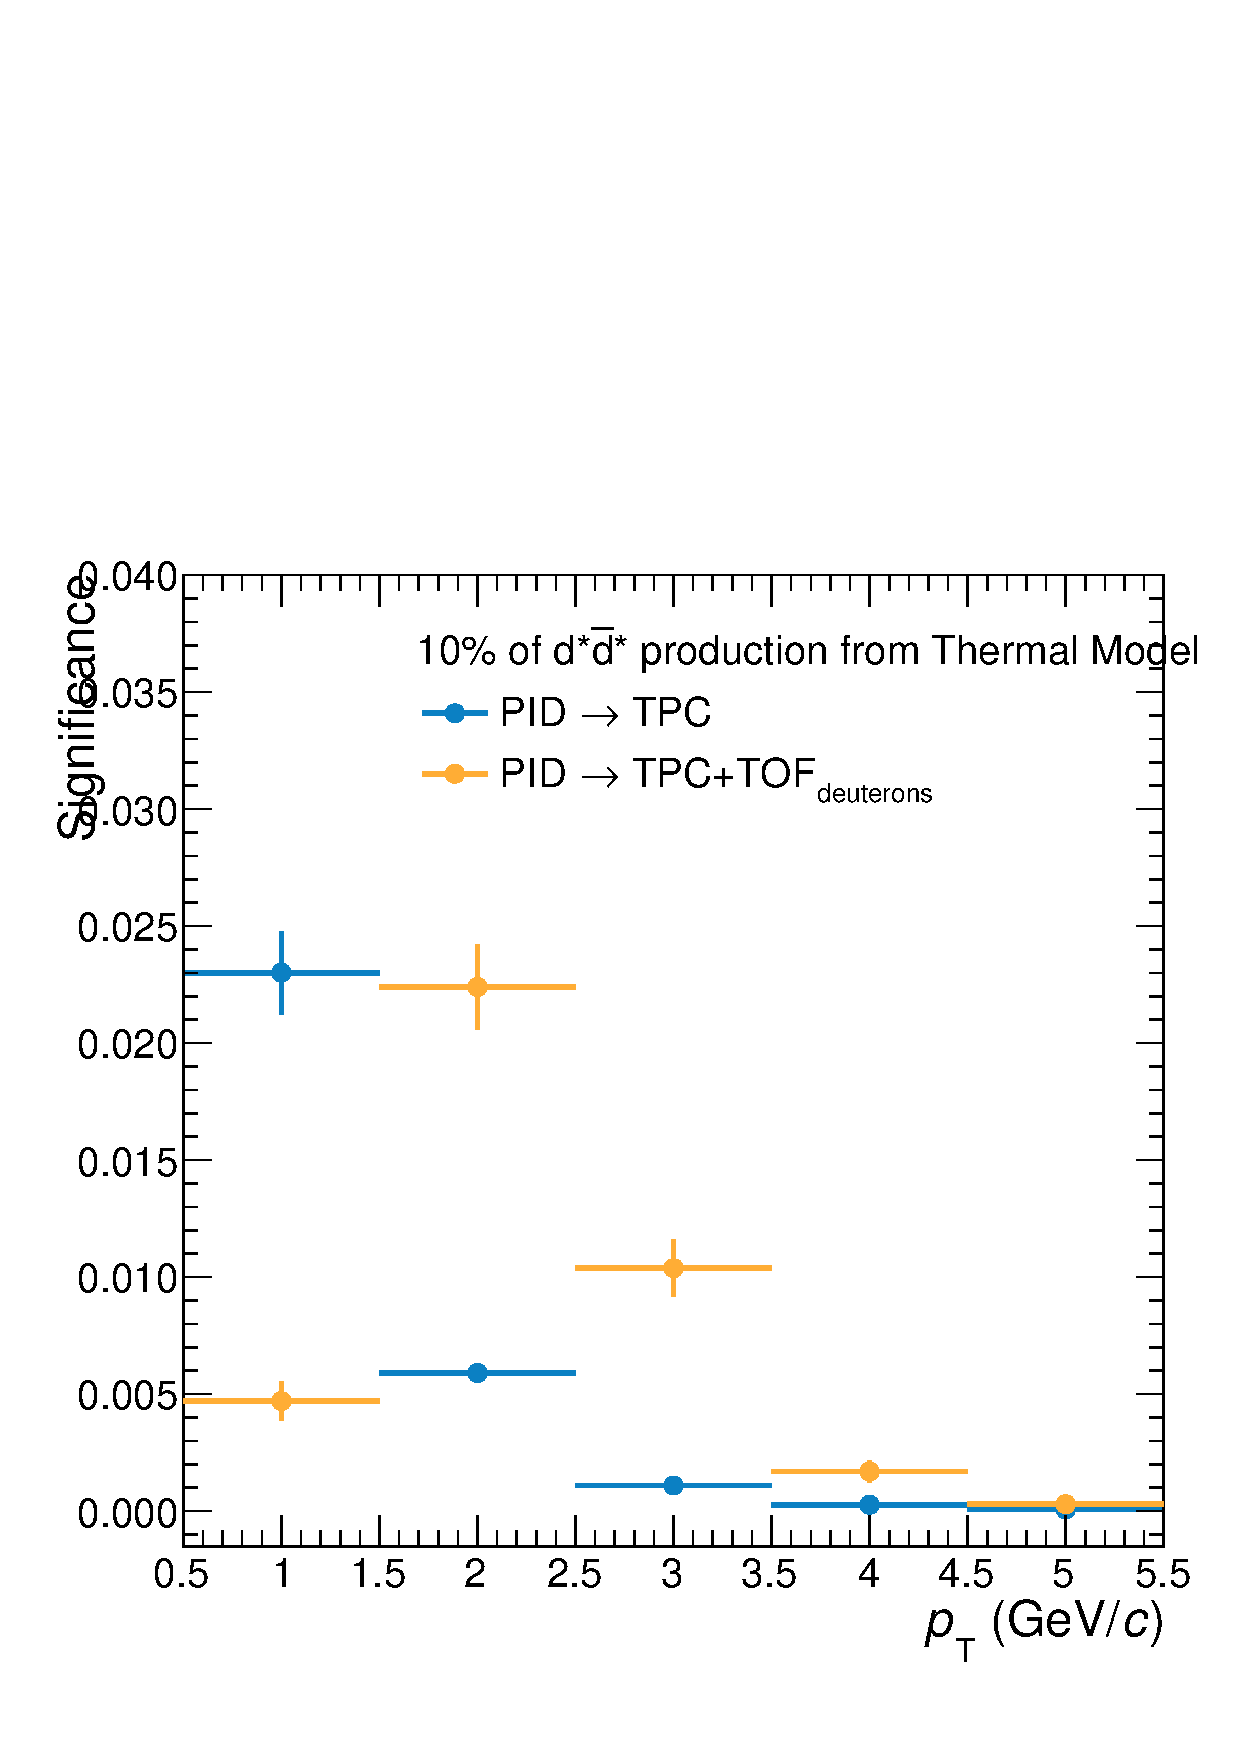
\includegraphics[width=\linewidth]{gfx/sig_0}
  \caption{}
  \label{fig:tem01}
\end{subfigure}%
\begin{subfigure}{.33\textwidth}
  \centering
  \captionsetup{justification=centering}
  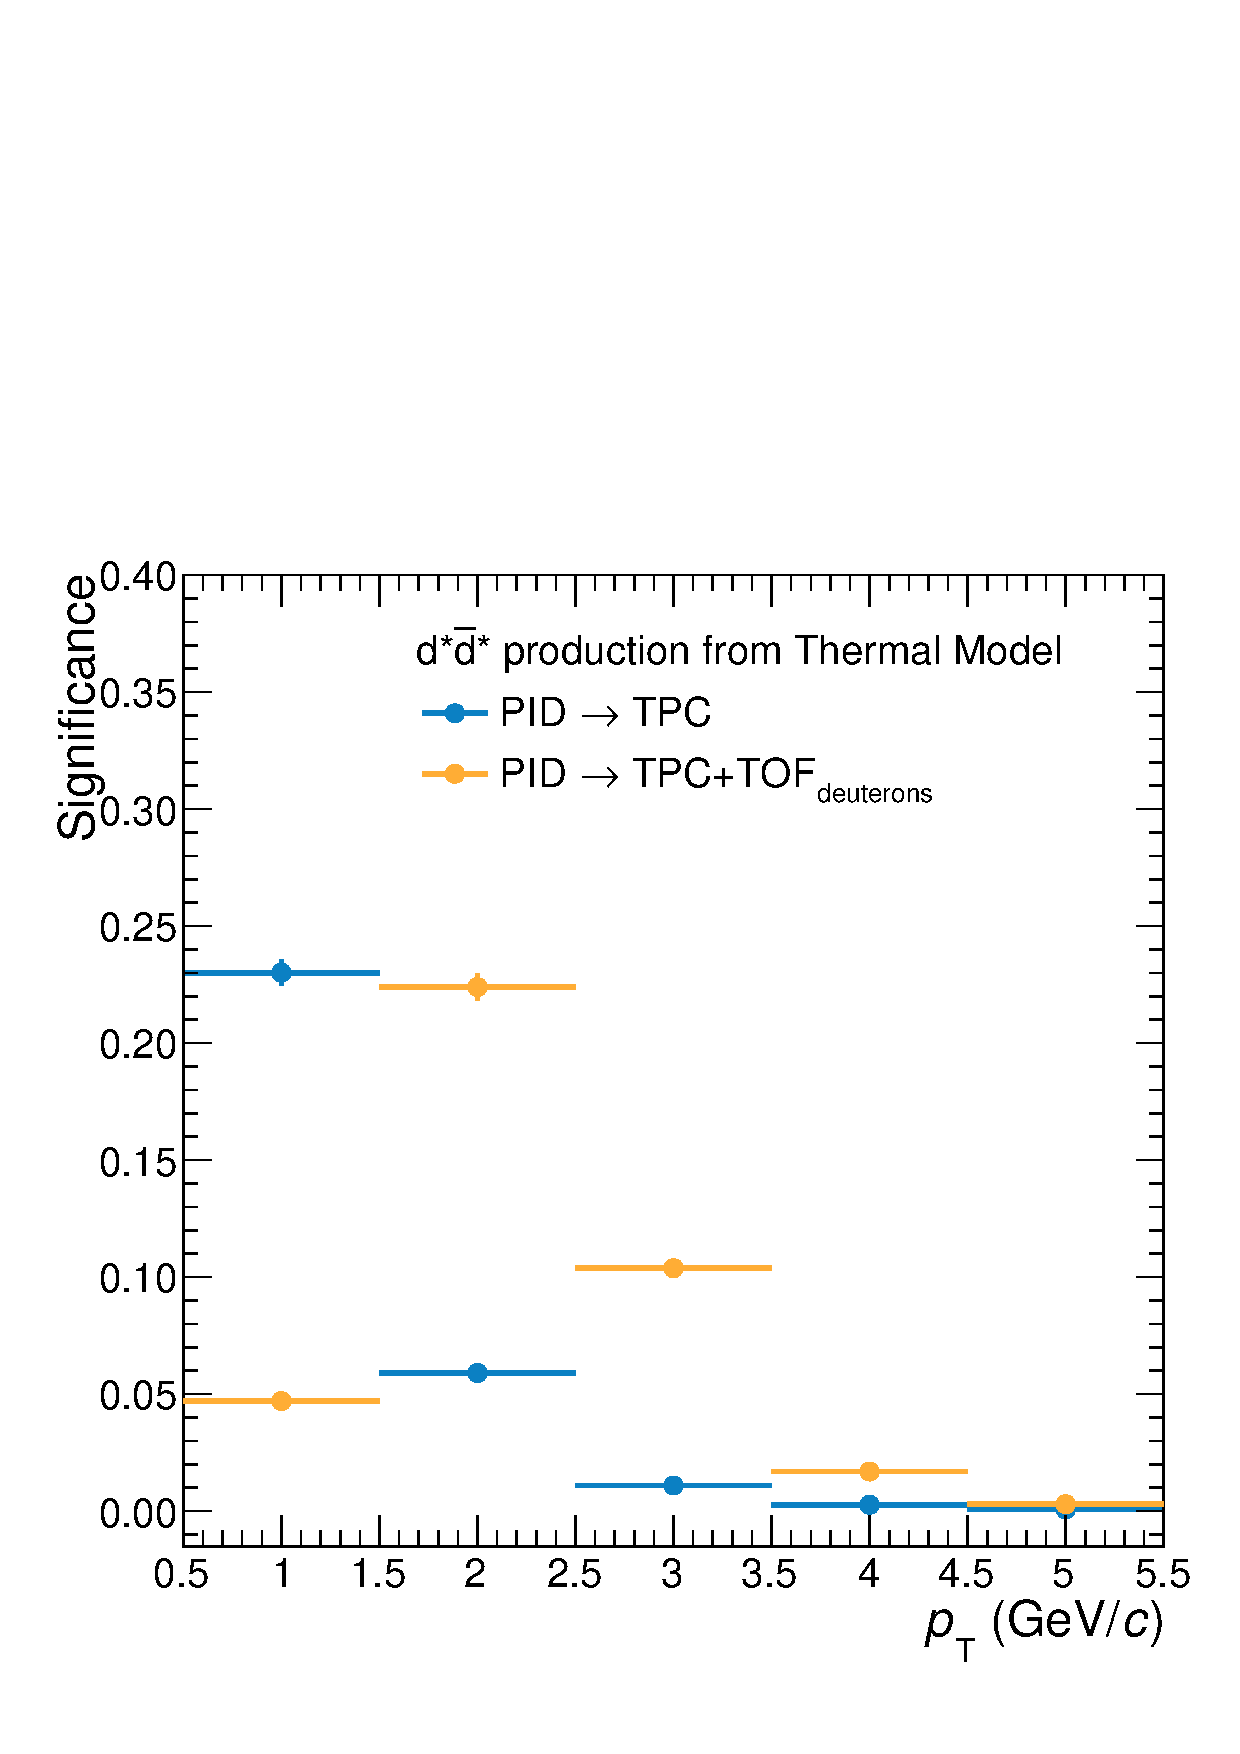
\includegraphics[width=\linewidth]{gfx/sig_1}
  \caption{}
  \label{fig:tem12}
\end{subfigure}
\begin{subfigure}{.33\textwidth}
  \centering
  \captionsetup{justification=centering}
  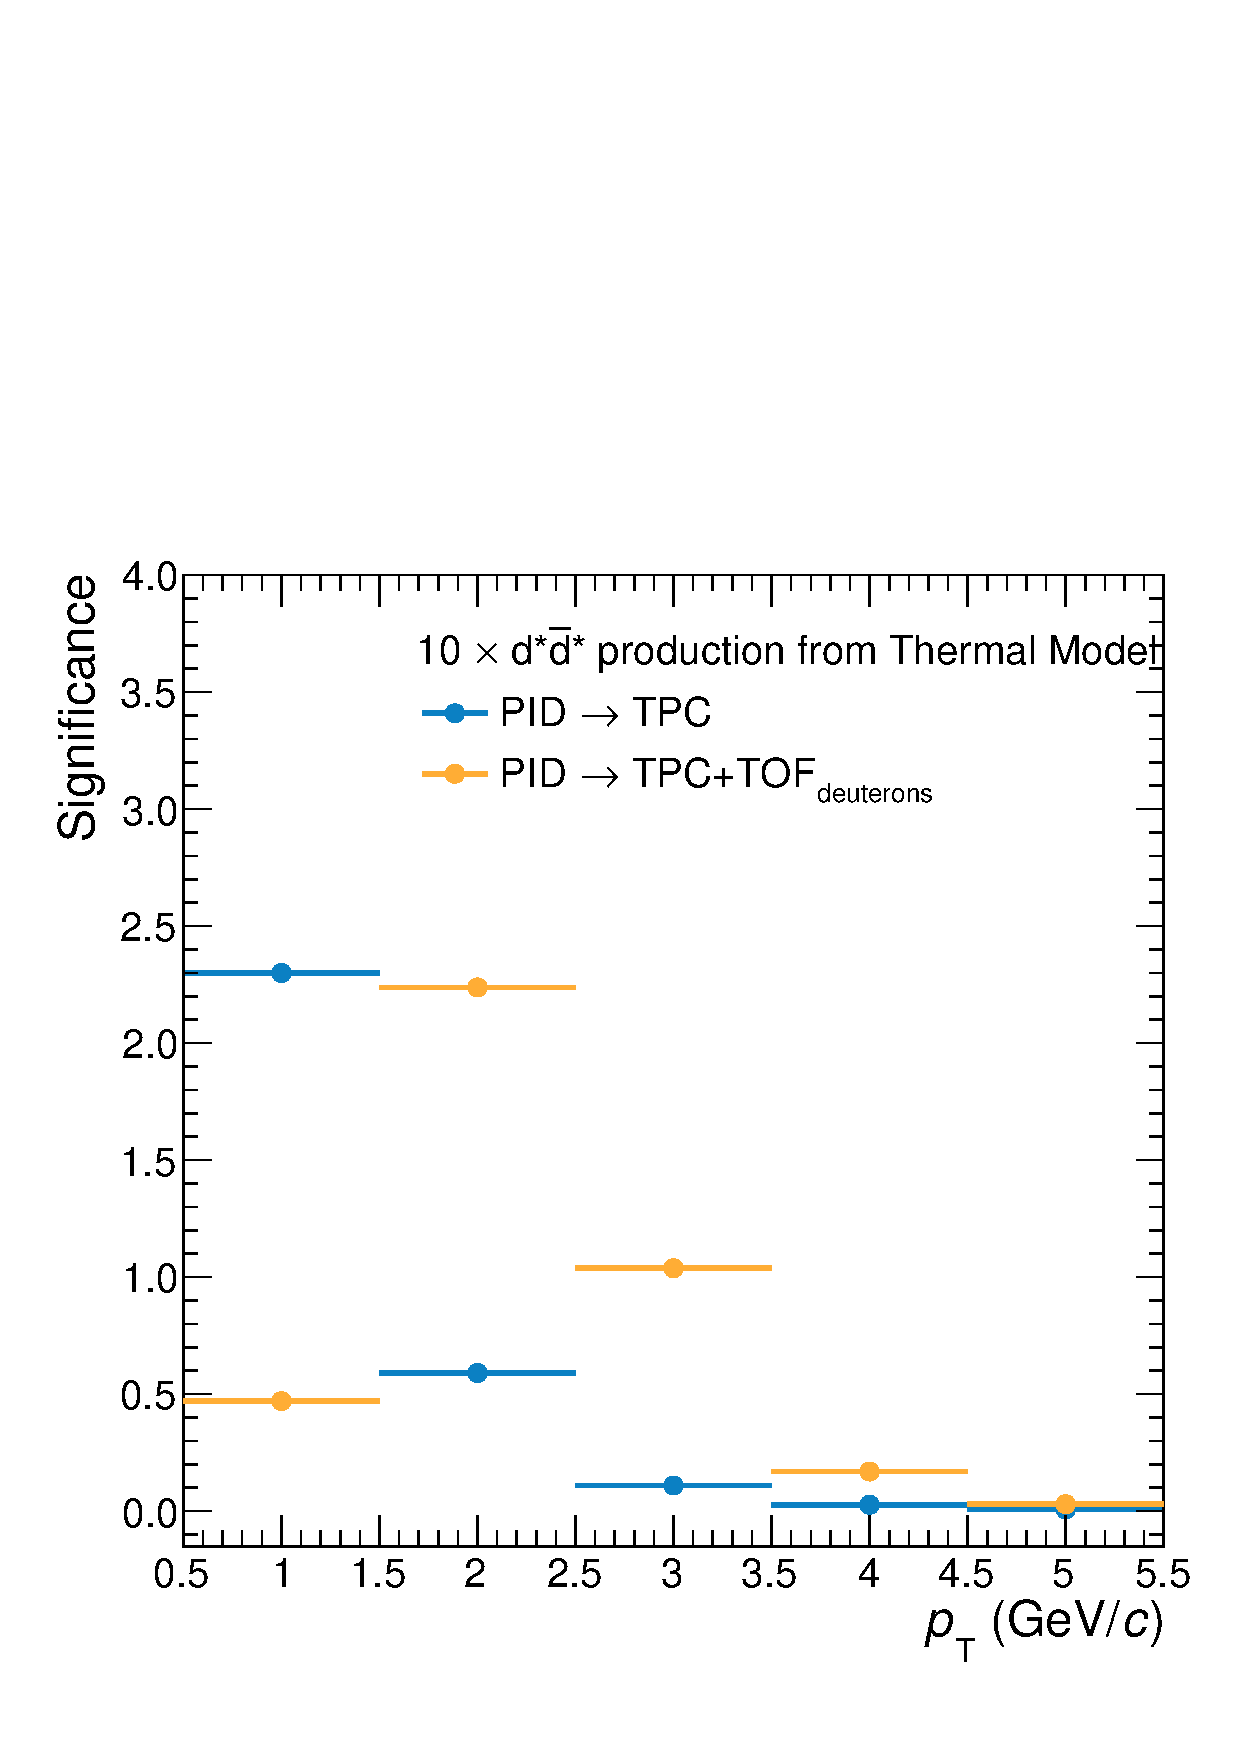
\includegraphics[width=\linewidth]{gfx/sig_2}
  \caption{}
  \label{fig:tem23}
\end{subfigure}
\caption{Significance of the measurement as a function of transverse momentum compared for the TPC and the TPC+TOF$_{deuteron}$ PID configurations.} % descrivere le 3 figure.}
\label{fig:tem01}
\end{figure}

The significance has been estimated by integrating signal and background in a 70 \mevcs wide region around the
mass peak of the \ds. Figure ~\ref{fig:} shows the significance in various \pt bins for both the TPC and the
TPC+TOF$_{deuteron}$ PID configurations.
The transverse momentum binning has been shifted specifically for this study: in the 0 to 0.5 \pT region the number of reconstructed d∗ is negligible with respect to the combinatorial background.

While in the first \pT bin the TPC only PID guarantees an optimal identification of pions and deuterons showing the 
maximum of significance, starting from 1.5 \gev the TPC+TOF$_{deuteron}$ configuration reduces the combinatorial background
and improves the significance. 
The wide peak of the \ds makes its identification challenging for the experimental condition at the LHC and if the thermal
model prediction is correct it is possible to set only an upper limit to the production cross section of \ds.


